%----------------------------------------------------------------
%
%  File    :  thesis.tex
%
%  Authors :  Keith Andrews, IICM, TU Graz, Austria
%             Manuel Koschuch, FH Campus Wien, Austria
% 
%  Created :  22 Feb 96
% 
%  Changed :  24 March 2009
% 
%----------------------------------------------------------------

% Please send any questions, comments, remarks or complaints to
% manuel.koschuch@fh-campuswien.ac.at


% --- General Setup ---------------------------------------------

\documentclass[12pt,a4paper,oneside]{book}

%\usepackage{times}

%\renewcommand{\rmdefault}{phv} % Arial
%\renewcommand{\sfdefault}{phv} % Arial

\usepackage{listings}	%% added to avoid the \lstlistoflistings error
\lstset{language=XML,
    frame=bottom, 
    linewidth=\columnwidth,
    breaklines=true,
    basicstyle=\tiny,
    }

\usepackage[utf8]{inputenc}   % so can use Umlaut chars  ä, ü
\usepackage[ngerman]{babel}
\usepackage[T1]{fontenc}

\usepackage[bf,sf]{subfigure}
\renewcommand{\subfigtopskip}{0mm}
\renewcommand{\subfigcapmargin}{0mm}

\usepackage{url}
\expandafter\def\expandafter\UrlBreaks\expandafter{\UrlBreaks\do\a%
\do\b\do\c\do\d\do\e\do\f\do\g\do\h\do\i\do\j\do\k\do\l\do\m\do\n%
\do\o\do\p\do\q\do\r\do\s\do\t\do\u\do\v\do\w\do\x\do\y\do\z\do\&}
\usepackage{latexsym}
\usepackage{ifpdf} % detect outputstyle
\usepackage{geometry} % define pagesize in more detail
\usepackage{fancyhdr} % nicer headers and footers
\usepackage{colortbl} %define colored backgrounds for tables
\usepackage{multicol}

\ifpdf
  \usepackage[pdftex]{graphicx}
  \DeclareGraphicsExtensions{.pdf,.jpg,.png}
  \pdfcompresslevel=9
  \pdfpageheight=297mm
  \pdfpagewidth=210mm
  \usepackage[         % hyperref should be last package loaded
    pdftex,
    bookmarks,
    bookmarksnumbered,
    linktocpage,
    pagebackref,
    pdfview={Fit},
    pdfstartview={Fit},
    pdfpagemode=UseOutlines,                 % open bookmarks in Acrobat
  ]{hyperref}
 
  \usepackage{bookmark}
\else                      % latex
  \usepackage{graphicx}
  \DeclareGraphicsExtensions{.ps}
\fi

\geometry{a4paper,left=30mm,right=25mm, top=30mm, bottom=30mm}

\setlength{\parskip}{3pt plus 1pt minus 0pt}       % vert. spacebeforeaparagraph

\setcounter{tocdepth}{1}        % lowest section level entered in ToC
\setcounter{secnumdepth}{2}     % lowest section level still numbered
% --- Start of Document ----------------------------------------

\begin{document}

\frontmatter
\normalsize
\pagestyle{empty}            % for title pages

%----------------------------------------------------------------
%
%  File    :  title.tex
%
%  Authors :  Keith Andrews, IICM, TU Graz, Austria
%             Manuel Koschuch, FH Campus Wien, Austria
% 
%  Created :  22 Feb 96
% 
%  Changed :  22 February 2011
% 
%----------------------------------------------------------------


% --- Main Title Page ------------------------------------------------

% A4 paper =  w=21cm, h=29.7cm

%\setlength{\textheight}{26.83cm}
%\setlength{\textwidth}{17cm}
%
%\setlength{\oddsidemargin}{-0.04cm}
%\setlength{\topmargin}{-2.5cm}

%\pagestyle{fancyplain}
%\fancyhead{}
%\renewcommand{\headrulewidth}{0.0pt}
%\fancyhead[L]{\includegraphics[height=25mm]{images/logo.png}}
%\fancyfoot[C]{\fancyplain}

\vspace*{-2.5cm}

\begin{center}

\vspace{1.3cm}

\hspace*{-1.0cm} {\Large \textbf{iOS Jailbreak\\}}

\hspace*{-1.0cm} und die Auswirkungen auf die Sicherheit und Vertrauenswürdigkeit des Systems \\

\vspace{2.2cm}

\hspace*{-1.0cm} \textbf{Diplomarbeit\\}

\vspace{0.65cm}

\hspace*{-1.0cm} Zur Erlangung des akademischen Grades \\

\vspace{0.65cm}

\hspace*{-1.0cm} \textbf{Master of Science in Engineering (MSc)\\}

\vspace{0.65cm}

\hspace*{-1.0cm} der Fachhochschule Campus Wien \\
\hspace*{-1.0cm} Masterstudiengang IT-Security \\

\vspace{5cm}

\hspace*{-1.0cm} \textbf{Vorgelegt von:} \\
\hspace*{-1.0cm} Michael Fuska, BSc \\

\vspace{0.65cm}

\hspace*{-1.0cm} \textbf{Personenkennzeichen}\\
\hspace*{-1.0cm} c1410537032 \\

\vspace{2.1cm}

\hspace*{-1.0cm} \textbf{Erstbegutachter/in:} \\
\hspace*{-1.0cm} Katharina Krombholz, MSc \\

\vspace{0.5cm}

\hspace*{-1.0cm} \textbf{Zweitbegutachter/in:} \\
\hspace*{-1.0cm} Dr. Martin Mulazzani, \\


\vspace{1.4cm}

\hspace*{-1.0cm} \textbf{Eingereicht am:} \\
\hspace*{-1.0cm} 07.08.2016 \\

\end{center}

\newpage

\pagestyle{empty}

\vspace*{16.5cm}  %% change from 17cm to 16.5cm to avoid an empty page

\hspace*{-0.7cm} \underline{Erklärung:}\\\\
Ich erkläre, dass die vorliegende Diplomarbeit von mir selbst verfasst wurde und ich keine anderen als die angeführten Behelfe verwendet bzw. mich auch sonst keiner unerlaubter Hilfe bedient habe.\\
Ich versichere, dass ich dieses Diplomarbeitsthema bisher weder im In- noch im Ausland (einer Beurteilerin/einem Beurteiler zur Begutachtung) in irgendeiner Form als Prüfungsarbeit vorgelegt habe.\\
Weiters versichere ich, dass die von mir eingereichten Exemplare (ausgedruckt und elektronisch) identisch sind.\\\\
Datum: \hspace{6cm} Unterschrift:\\






              % Title Page

\pagestyle{fancy} 
\fancyhf{}
	
\setlength{\headheight}{15pt}
\renewcommand{\headrulewidth}{0.0pt}

\fancyfoot[R]{\thepage}      
\pagenumbering{roman}        % for preliminary pages

%%----------------------------------------------------------------
%
%  File    :  acknowl.tex
%
%  Authors :  Keith Andrews, IICM, TU Graz, Austria
%             Manuel Koschuch, FH Campus Wien, Austria
% 
%  Created :  22 Feb 96
% 
%  Changed :  30 Oct 2008
% 
%----------------------------------------------------------------

\begin{center}
{\Large\bfseries Danksagung}
\end{center}

(Falls gewünscht.)          % Acknowledgements
%----------------------------------------------------------------
%
%  File    :  abstracts.tex
%
%  Authors :  Keith Andrews, IICM, TU Graz, Austria
%             Manuel Koschuch, FH Campus Wien, Austria
% 
%  Created :  22 Feb 96
% 
%  Changed :  30 Oct 2008
% 
%----------------------------------------------------------------


% --- German and English Abstracts ------------------------------------------------

% --- German Abstract ----------------------------------------------------
\cleardoublepage

\begin{center}
{\Large\bfseries Kurzfassung}
\end{center}


(Z.B. ``Diese Arbeit beschäftigt sich mit...'')


% --- English Abstract ----------------------------------------------------

\cleardoublepage

%\selectlanguage{english}

\begin{center}
{\Large\bfseries Abstract}
\end{center}

(E.g. ``This thesis deals with...'')

%\selectlanguage{austrian}
        % Englisch and German abstracts
%----------------------------------------------------------------
%
%  File    :  glossary.tex
%
%  Author  :  Manuel Koschuch, FH Campus Wien, Austria
% 
%  Created :  30 Oct 2008
% 
%  Changed :  30 Oct 2008
% 
%----------------------------------------------------------------

\begin{center}
{\Large\bfseries Begriffsdefinition Verzeichnis}
\end{center}

\begin{table*}[htbp]
    \begin{center}
      \begin{tabular}{p{3cm}p{12cm}} 
        
        \textbf{App Store} &  Der Begriff App Store bezeichnet einen Online Store, welcher es ermöglicht, Apps herunterzuladen und zu installieren\\ 
        
        \textbf{Backdoor} &  Eine Backdoor bezeichnet einen Teil einer Software, der es dem User ermöglicht, unter Umgehung der normalen Zugriffssicherung Zugang zum iOS Device zu erhalten.\\
        \textbf{Bug} &  Als Bug wird ein Fehlverhalten von Computerprogrammen bezeichnet.\\ 
		
		\textbf{Cleartext} &  Als Cleartext werden Daten bezeichnet, die ohne weitere Bearbeitung (entschlüsseln) verarbeitet/gelesen werden können\\     
		
		\textbf{Framework} & Ein Framework ist ein Programmiergerüst, das im Rahmen der objektorientierten Softwareentwicklung verwendet wird. \\
		
		\textbf{Hacker} &  Der Begriff Hacker wird verwendet, wenn eine Person oder ein System versucht, Zugriff auf ein fremdes System unerlaubt zu erhalten.\\
		\textbf{Hook} & Der Begriff Hook beschreibt in der Softwareentwicklung eine Programmschnittstelle.\\
		  
		\textbf{iOS} &  Der Begriff iOS steht für das mobile Apple Betriebssystem.\\
		  
		 \textbf{Jailbreak} &  Als Jailbreak wird das nicht-autorisierte Entfernen von Nutzungsbeschränkungen bei iOS Geräten bezeichnet.\\  
		 \textbf{Kernelspace} & Der Begriff Kernelspace beschreibt einen Bereich im virtuellen Memory, in dem nur privilegierte Prozesse des Betriebssystems laufen.\\ 
		      
		  \textbf{Malware} &  Als Malware wird eine Schadsoftware bezeichnet, die unerwünschte bzw. schädliche Programme ausführt.\\
		 
		  \textbf{proc-Struktur} & Ist ein virtuelles Filesystem, in dem alle \textit{\glqq runtime\grqq{}} Prozess-Informationen gespeichert werden.\\
		  
		  \textbf{Userspace} & Der Begriff Userspace beschreibt einen Bereich im virtuellen Memory, in dem auch nicht privilegierte Prozesse des Betriebssystems laufen.\\
		  
		 \textbf{Root-Rechte} &  Der Begriff Root-Recht steht für den uneingeschränkten Zugriff auf das Betriebssystem und auf die Device Ressourcen hat.\\
		 \textbf{Root-User} &  Als Root-User bezeichnet man den User, der uneingeschränkten Zugriff auf das Betriebssystem und auf die Device Ressourcen.\\ 
		 \textbf{Zero Day Bug} &  Der Begriff Zero Day Bug steht für einen Softwarefehler, der bis jetzt noch nicht veröffentlicht wurde und den Hackern noch zur Verfügung steht.\\
		  
		\end{tabular}		    
    \end{center}
\end{table*} 
%----------------------------------------------------------------
%
%  File    :  glossary.tex
%
%  Author  :  Manuel Koschuch, FH Campus Wien, Austria
% 
%  Created :  30 Oct 2008
% 
%  Changed :  30 Oct 2008
% 
%----------------------------------------------------------------

\begin{center}
{\Large\bfseries Abkürzungsverzeichnis}
\end{center}

\begin{table*}[htbp]
		 \begin{tabular}{p{3cm}p{12cm}} 
		    \textbf{AES} & Advanced Encryption Standard \\
            \textbf{AES-CBC} & Advanced Encryption Standard Cipher Block Chaining \\
            \textbf{AES-XTS} & Advanced Encryption Standard XEX-based tweaked-codebook mode with ciphertext stealing \\ 
		     \textbf{ASLR} & Address space layout randomization \\
		     \textbf{AFC} & Apple File Conduit\\
		     
		     \textbf{BYOD} & Bring Your Own Device\\
		     
		     \textbf{CTR-DRBG} & Counter mode Deterministic Random Byte Generator \\
		     
		     \textbf{DFU Mode} & Device Firmware Upgrade Mode\\
		     \textbf{DDI} & Development Disk Image \\
		     \textbf{DMA} & Direct Memory Access\\
		     \textbf{DTLS} & Datagram Transport Layer Security \\
		     
		     \textbf{GID} & Group ID \\
		     \textbf{GQM} & Goal Question Metric Methode \\
		     
		     \textbf{HTML} & Hypertext Markup Language \\
		     
		     \textbf{IPsec} & Internet Protocol Security \\
		     \textbf{iOS} & iPhone Betriebssystem\\
		     
		     
		     \textbf{MDM} & Mobile Device Management \\
		     
		     \textbf{NFC} & Near Field Communication \\
             
             \textbf{JIT} & Just In Time \\		     
		     
		     \textbf{SGML} & Standard Generalized Markup Language \\
 		     
 		     \textbf{TLS} & Transport Layer Security \\
 		     
 		     \textbf{UID} & Unique ID \\
 		     
 		     \textbf{RNG} & Random Number Generator\\
 		     \textbf{RPC} & Remote Procedure Call \\
 		     
 		     \textbf{UDID} & Unique Device Identifiers\\
 		     \textbf{UUID} &  Universally Unique IDentifier \\
 		 	 
 		 	 \textbf{VPN} & Virtual Private Network \\
		\end{tabular}
\end{table*}         % Glossary
%----------------------------------------------------------------
%
%  File    :  keywords.tex
%
%  Author  :  Manuel Koschuch, FH Campus Wien, Austria
% 
%  Created :  30 Oct 2008
% 
%  Changed :  30 Oct 2008
% 
%----------------------------------------------------------------

\begin{center}
{\Large\bfseries Schlüsselbegriffe}
\end{center}

\noindent
\textbf{iOS Sicherheitsmechanismen } \\
\textbf{Jailbreak } \\
       % Keywords
%----------------------------------------------------------------
%
%  File    :  toc.tex
%
%
%  Authors :  Keith Andrews, IICM, TU Graz, Austria
%             Manuel Koschuch, FH Campus Wien, Austria
% 
%  Created :  22 Feb 96
% 
%  Changed :  30 Oct 2008
% 
%----------------------------------------------------------------

{
\setlength{\parskip}{3pt plus 3pt minus 3pt}     % compact table of contents

\tableofcontents
}
                 % Table of Contents

\mainmatter

\cleardoublepage
\renewcommand{\headrulewidth}{0.4pt}

\pagestyle{fancy}            % for main pages
\fancyhf{}
\fancyhead[RO]{\slshape \nouppercase{\leftmark}}
\fancyfoot[R]{\thepage}     
\pagenumbering{arabic}      % for main pages

%--- Include your chapters here ----------

%----------------------------------------------------------------
%
%  File    :  chapter1.tex
%
%  Authors : Michael Fuska, FH Campus Wien, Austria% 
%  Created : 13 Feb 2016
%
%  Changed :  
% 
%----------------------------------------------------------------


\chapter{Einleitung}
\label{ch:intro}


\section{Einführung}
\label{sec:Einführung}

Das Smartphone ist ein ständiger Begleiter des Menschen geworden. Es nimmt von Tag zu Tag mehr Einfluss auf unser Leben. Neben dem privaten Gebrauch ist es auch im beruflichen Alltag nicht mehr wegzudenken. Sensible Informationen und Daten werden auf dem Smartphone verarbeitet und/oder gespeichert. Daraus ergibt sich, dass die Sicherheit und Stabilität der Smartphones zunehmend an Bedeutung gewinnen muss.\par 
Am 29.Juni 2007 wurden das erste iPhone mit der iOS Version 1.0 von Apple zum Verkauf angeboten. Elf Tage nach Verkaufsstart war der erste Jailbreak für diese iOS Version verfügbar. Das Ziel eines Jailbreak ist es, \textit{\glqq Root-Zugriffsrechte\grqq{}} für das Betriebssystem zu erhalten. Der \textit{\glqq Root-User\grqq{}} hat vollen Zugriff auf das Betriebssystem und kann mit diesen Rechten unter anderem, unautorisierte Software auf dem iOS Device installieren.\par 

Es gibt für \textit{\glqq gejailbreakte\grqq{}} iOS Devices, neben dem offiziellen App Store (Apple), zwei weitere App Stores
\begin{itemize}
    \item Cydia
    \item Taig
\end{itemize}
Diese beiden App Stores unterliegen nicht der Sicherheitsüberprüfung von Apple. Der User muss sich über die möglichen Konsequenzen bewusst sein, wenn er eine Applikation aus einem nicht offiziellen App Store installiert. Neben Malware, die direkt in der heruntergeladen und installierten App eingebettet sein kann, ermöglichen Programme wie 
\begin{itemize}
    \item SSH Dämon,
    \item Terminalprogramm,
    \item und Shells (sh, bash)
\end{itemize}
weitere Angriffsvektoren für \textit{\glqq Hacker\grqq{}}.

Ein Jailbreak nutzt \textit{\glqq Bugs\grqq{}} im iOS aus und umgeht so die Sicherheitsmaßnahmen von Apple. Für Apple bedeutet jeder Jailbreak ein Aufzeigen von Sicherheitsschwächen des Apple Betriebssystems. Durch den öffentlichen Druck und die Möglichkeit, dass diese Sicherheitsmängel für Angriffe ausgenutzt werden könnten, wird Apple immer wieder gezwungen, Zeit und Geld in die Verbesserung der iOS Sicherheit zu investieren. 

Am 21.September 2015 wurde von der Firma \textit{\glqq Zerodium\grqq{}} ein Preisgeld von einer Million U.S Dollar für einen \textit{\glqq zero day bug\grqq{}} für die iOS Version 9.x ausgeschrieben. Das Ziel dieser Ausschreibung war es, einen System Remote-Zugriff zu erhalten. 
\begin{description}
    \item[\parbox{\textwidth} {Folgende iOS Sicherheitsmechanismen mussten durch diesen Jailbreak umgangen werden}]~\par
    \begin{enumerate}
        \item ASLR, 
        \item Sandbox,
        \item Root Zugriff, 
        \item Code Signing, 
        \item und der Secure Boot Chain.
    \end{enumerate}
\end{description} 

Dieser unerlaubte Zugriff auf das Smartphone musste vor dem User verborgen bleiben. Diese Ausschreibung zeigt, dass nur mehr sehr wenige Menschen die Fähigkeiten besitzen, Sicherheitslücken des mobilen Betriebssystems von Apple auszunützen. Am ersten November 2015 endete die Ausschreibung und es wurde bekanntgegeben, dass das Preisgeld einmal ausbezahlt wurde. 

Am 29.September 2015 nahm Apple Stellung  zu den \textit{\glqq backdoor\grqq{}} Gerüchten in der Presse. Laut Aussage von Apple gibt es ab der iOS Version 8 keine Möglichkeit mehr, an die \textit{\glqq Cleartext Userdaten\grqq{}} eines Devices zu gelangen. Apple begründet dies in ihrer Aussendung so:
\begin{enumerate}
    \item \textbf{Es gibt für Apple keine Möglichkeit, den Passcode des iOS Devices zu umgehen.}
    \item \textbf{Die Verschlüsselungskeys werden von Apple nicht mehr gespeichert.}
\end{enumerate}

Diese Ausgabe wird durch einen weiteren Fall untermauert. Das FBI forderte im Dezember 2016 Apple auf, dem FBI zu helfen und eine iOS Device zu entsperren. Das FBI benötigte einen Zugang zu den Userdaten des Gerätes. Selbst die in diesem Fall vertrauten Gerichte, konnten Apple nicht verpflichten, das iPhone zu entsperren. Zur Zeit arbeitet der US Kongress an einem neuem Gesetzt, in dem festgelegt werden soll, wie mit solchen Fällen umgegangen werden soll. Ein Teil dieser Arbeit wird es sein, festzulegen, ob Firmen wie Apple gezwungen werden können, \textit{\glqq Backdoors\grqq{}} in ihrer Software zu implementieren. Dies würde es staatlichen Organisation erleichtern, Zugriff auf die Daten von Usern erhalten, dies hat den Beigeschmack, dass dieses Backdoor auch von jedem anderen benutzt werden kann, sobald dieser, das Backdoor entdeckt würde. 

\section{Motivation }
\label{sec:IntroMotivation}
Das iPhone ist nun seit über sechs Jahren mein ständiger Begleiter, sowohl im privaten als auch im beruflichen Umfeld. Die unzureichende Möglichkeit das iPhone meinen Bedürfnissen anzupassen, war ausschlaggebend für mich, mich mit dem Thema iOS Jailbreak auseinander zusetzten. 
Für mich ist weiters wichtig, dass nach der Installation eines Jailbreaks die klassischen Ziele der Informationssicherheit
\begin{enumerate}
    \item die \textbf{Integrität,}
    \item die \textbf{Vertraulichkeit} 
    \item und die \textbf{Verfügbarkeit der Daten,}
\end{enumerate}
sowie die \textbf{Stabilität des System} erhalten bleiben.


\section{Aufbau dieser Arbeit}
\label{sec:IntroAufbau}
In dieser Sektion wird der Aufbau der Arbeit beschrieben. \textbf{Das Kapitel \ref{ch:intro}} befasst sich mit einer allgemeinen Beschreibung des Themas, unteranderem gibt es einen Überblick bzw. Einblick in die weiteren Kapiteln dieser Arbeit. Des weiter wird die empirische Methode erklärt mit der die erhoben Daten aufbereitet und analysiert werden. 

\paragraph{Im Kapitel \ref{ch:JB}} werden die unterschiedlichen Arten von Jailbreaks beschrieben, sowie statistische Aufbereitung zu diesem Thema.

\paragraph{Im Kapitel \ref{ch:iOS}} wird das mobile Betriebssystem von Apple im Detail beschrieben. Es werden die Betriebssystemanforderungen auf den unterschiedlichen Layer des mobilen Betriebssystem von Apple eingegangen. Die iOS Architektur wird in diesem Kapitel im Detail erklärt. 

\paragraph{Im Kapitel \ref{ch:iOSSicherheitsKonzepte}} werden die einzelnen iOS Sicherheitsmechanismen beschrieben die von Apple im Laufe Zeit implementiert worden sind.

\paragraph{Im Kapitel \ref{ch:Ergebnisse}} werden die Daten anhand der im Kapitel \ref{ch:intro} definierten Fragestellungen aufbereitet. Die Zielfragestellungen die im Kapitel \ref{ch:intro} angeführt wurden, werden mit den erstellten Metriken zu den Fragestellungen beantwortet.

\paragraph{Im Kapitel \ref{ch:Conclusion}} werden die Ergebnisse zusammengefasst und es werden die daraus resultieren Schlüsse dokumentiert.

\section{Methodik dieser Arbeit}
\label{sec:MethArbeit}
In dieser Arbeit wird die Goal Question Metric (GQM) Methode zur Analyse der erhoben Daten herangezogen. Die GQM Methode ist eine systematische Vorgehensweise zur Erstellung spezifischer Qualitätsmodelle im Bereich der Softwareentwicklung. Hierbei ist vor allem die klar strukturierte Vorgehensweise dieses Systems hervorzuheben. Dies hat zur Folge, dass die Ergebnisse dieser Arbeit Nachvollziehbar und leicht Beweisbar sind.

\begin{description}
    \item[\parbox{\textwidth} {Die GQM-Methode ist in drei Schritte unterteilt und dient zur Bewertung der erhoben Daten}]~\par
    \begin{enumerate}
        \item Die Definition des Ziels(Goals)
        \item Die Definition der Fragen, deren Beantwortung aussagt, ob das Ziel erreicht wurde (Questions)
        \item Die Definition der Metriken, die eine messbare Beantwortung der Fragen darstellen(Metrics)
    \end{enumerate}
\end{description} 

\subsection{GQM - Goal Definition}
\label{sec:GQMGoal}

\paragraph{G1:} \textit{\glqq Das Ziel dieser Arbeit ist es eine Aussage über die Sicherheit und die Vertrauenswürdigkeit der iOS Produkte(iPhone, iPad) tätigen zu können.\grqq{}}
\paragraph{G1.1:} \textit{\glqq Erstes abgeleitetes Ziel ist es einen Zusammenhang zwischen der Sicherheit und der Vertrauenswürdigkeit des iOS Device und der verwenden Hardware der iOS Geräte herzustellen.\grqq{}}

\paragraph{G1.2:} \textit{\glqq Zweites abgeleitetes Ziel dieser Arbeit ist es einen Zusammenhang zwischen der Sicherheit und der Vertrauenswürdigkeit des iOS Device und der installierten iOS Software herzustellen.\grqq{}}

\subsection{GQM - Fragen Definition}
\label{sec:GQMFragen}

\paragraph{Q1:} \textit{\glqq Welche Faktoren sind für die Sicherheit und die Vertrauenswürdigkeit eines iOS Device ausschlaggebend (Kapitel: \ref{sec:Frage1})?\grqq{}}
                    
 \paragraph{Q2:} \textit{\glqq Welche Auswirkung haben die von Apple eingeführten Sicherheitsmechanismen und Sicherheitsupdates auf die Sicherheit des Systems (Kapitel: \ref{sec:Frage2})?\grqq{}}
        
\subsection{Hypothese}
\label{sec:GQMHypothese}
\paragraph{H1:} \textit{\glqq Die Anzahl der Tage, die die JB Community benötigt, um ein JB für eine iOS Version oder ein iOS Device zu veröffentlichen, kann als Indikator für die Sicherheit und Vertrauenswürdigkeit der iOS Produkte herangezogen werden.\grqq{}}

\subsection{GQM - Metrik Definition}
\label{sec:GQMMetrik}

Damit die Softwarequalität messbar gemacht werden kann, wurden unterschiedliche Modelle für diesen Prozess entwickelt. Im ISO Standard ISO/IEC 25010:2011 werden die unterschiedlichsten Softwaremerkmale definiert und festgehalten. \cite{IOS25010} Unter anderem werden die Merkmale für die Zuverlässigkeit einer Software in diesem Standard definiert. Ein Software-Sicherheitsmerkmal ist die Anzahl der Softwarebugs die in einer Software gefunden worden sind. In dieser Arbeit werden die geschlossenen Bugs der Apple-Sicherheitsupdates für diese Metrik herangezogen.
\begin{description}
    \item[\parbox{\textwidth} {In dieser Arbeit werden zwei Arten von Bugs unterschieden, die in den iOS Sicherheitsupdates geschlossen werden}]~\par
    \begin{enumerate}
        \item Softwarebugs die in JB verwendet wurden, um ein JB auf einer früheren iOS Versionen durchzuführen. 
        \item Softwarebugs die von Apple und anderen Sicherheitsforschern entdeckt und gemeldet wurden.
    \end{enumerate}
\end{description} 
 \par
Der zweite Ansatz bezieht sich auf die Anzahl der Tage die benötigt wurden, um für eine neue iOS Version ein JB zu veröffentlichen. Hierfür werden nur \textit{\glqq untethered Jailbreak Daten\grqq{}} verwendet, damit ist die Vergleichbarkeit der Daten in dieser Arbeit gewährleistet. \par 
Es werden in dieser Arbeit zwei Arten von Metriken für die Aufbereitung der Daten verwendet.
\begin{enumerate}
    \item \textit{\glqq External metrics\grqq{}}\\
    Diese Art der Metrik ermöglicht es die laufende Software von extern zu bewerten.
    \item \textit{\glqq Quality in use metrics\grqq{}} \\
    Diese Art der Metrik ermöglicht es eine finale Softwareversion zu bewerten. Dies ermöglicht es die finale Softwarequalität zu bewerten.
\end{enumerate}


%\section{Rahmenbedingungen}
%\label{sec:Rahmenbedingungen}
%In diesen Kapitel werden die Rahmenbedingungen für diese Arbeit zusammengefasst. Die Daten wurden von  unterschiedlich Quellen 
%\begin{description}
%    \item[\parbox{\textwidth} {Es werden nur folgenden}]~\par
%    \begin{enumerate}
%        \item  iOS Produkte betrachtet: iPhone 1 bis iPhone SE (Siehe Tabelle: \ref{tab:iOSHW})
%        \item iOS Version betrachtet: iOS Version 3.0 bis 9.3.2
%        \item JBs betrachtet. JBs die bis zum 01.07.2016 veröffentlicht wurden.
%    \end{enumerate}
%  \end{description} 
%








              % Einleitung
%%----------------------------------------------------------------
%
%  File    :  chapter2.tex
%
%  Authors :  Keith Andrews, IICM, TU Graz, Austria
%             Manuel Koschuch, FH Campus Wien, Austria
% 
%  Created :  22 Feb 96
% 
%  Changed :  30 Oct 2008
% 
%----------------------------------------------------------------


\chapter{Jailbreak}
\label{ch:JB}

\section{Allgemein}
\label{sec:JBAllgemein}

\section{Arten von Jailbreaks}
\label{sec:JBArten}

\subsection{Tethered Jailbreak}
\label{sec:JBTethered}

\subsection{Untethered Jailbreak}
\label{sec:JBUnTethered}

\subsection{Semi-Tethered Jailbreak}
\label{sec:JBSemiTethered}

\section{Jailbreak History}
\label{sec:JBHistory}

\section{Aufbau Jailbreak 9.2.1}
\label{sec:JBAufbau}

\subsection{Breaking out of the sandbox}
\label{sec:JBStep1}

\subsection{Obtaining arbitrary (unsigned) code execution}
\cite{TaiG[1]}
\cite{TaiG[2]}
\cite{TaiG[3]}

\label{sec:JBStep2}

\subsection{Obtaining root}
\label{sec:JBStep3}

\subsection{Patching the Kernel}
\label{sec:JBStep4}
          % Forensic
%----------------------------------------------------------------
%
%  File    :  chapter3.tex
%
%  Authors : Michael Fuska, FH Campus Wien, Austria
% 
%  Created : 13 Feb 2016
%
%  Changed :  
% 
%----------------------------------------------------------------


\chapter{Jailbreak}
\label{ch:JB}

% ------------- JB Allgemein --------------------
\section{Allgemein}
\label{sec:JBAllgemein}

Ein Jailbreak ermöglicht es dem User, die von Apple
vorgesehen Sicherheitsvorkehrung zu umgehen 
Der User erhält durch einen Jailbreak \glqq Zugriff\grqq{} auf das
Betriebsystem und die \glqq Root Zugriffsrechte \grqq{} des Betriebssystem.
Dadurch hat der User die Möglichkeit Applikationen zu installieren,
die nicht von Apple signiert worden sind. 
Mit einem Jailbreak steht dem User, zwei weitere \glqq Application Stores
\grqq{} zur Verfügung.

\begin{description}
\item[Von Apple nicht autorisierte \glqq Applikation Stores\grqq]~\par
	\begin{enumerate}
	   	\item \textbf{Cydia} \cite{Cydia[1]}
		\item \textbf{TaiG}
	\end{enumerate}
\end{description}

% ------------- Arten JB --------------------
\section{Arten von Jailbreaks}
\label{sec:JBArten}
Abhängig von der Art wie sich das iOS Device nach einem Jailbreak verhält, wenn
es rebooted wird, unterscheidet man die Arten von Jailbreaks. 

% ------------- Tethered Jailbreak--------------------
\subsection{Tethered Jailbreak}
\label{sec:JBTethered}
Bei einem \glqq tethered Jailbreak\grqq{} startet das iOS Device nicht nach
einem Reboot. Das iOS Device befindet sich nach einem Reboot im DFU Mode.
Damit das iOS Device wieder gebootet werden kann, muss dieses an einen PC
angeschlossen werden und mithilfe des Jailbreaktools neugestartet werden.

\begin{description}
\item[Zwei Beispiele für \glqq Tethered Jailbreaks\grqq{} sind]~\par
	\begin{itemize}
        \item \textbf{redsn0w}
        \item \textbf{Blackra1n}
    \end{itemize}
\end{description} 

% ------------- Semi Tethered Jailbreak--------------------
\subsection{Semi Tethered Jailbreak}
\label{sec:JBSemiTethered}

Bei einem \glqq Semi Tethered Jailbreak\grqq{} ist es möglich das iOS Device
zu rebooten. Das System startet nicht in den DFU Mode, sondern es ist
mit Einschränkung funktionsfähig. Safari, Mail, Cydia und alle Apps die über
Cydia installiert wurden funktionieren nicht. Das ausführen einer schon
installierten App ermöglicht es dem User, das iOS in einen normalen Zustand zu
bringen. Danach ist das iOS Device vollständig funktionsfähig.

\begin{description}
\item[Ein Beispiel für einen \glqq Semi Tethered Jailbreak\grqq{} ist]~\par
	\begin{itemize}
        \item \textbf{SemiTether (Cydia package)}
    \end{itemize}
\end{description} 

% ------------- UnTethered Jailbreak--------------------
\subsection{Untethered Jailbreak}
\label{sec:JBUntethered}

Bei einem \glqq untethered Jailbreak\grqq{} startet das iOS Device nach einem
Reboot ohne weitere Hilfsmittel.  
\begin{description}
\item[Einige Beispiele für \glqq untethered Jailbreaks\grqq{} sind]~\par
	\begin{multicols}{2}
	\begin{itemize}
        \item \textbf{Absinthe}
        \item \textbf{evasi0n7}
        \item \textbf{Pangu}
        \item \textbf{Pangu8}
        \item \textbf{Pangu9}
        \item \textbf{TaiG}
    \end{itemize}
    \end{multicols}
\end{description} 

% ------------- Semi Untethered Jailbreak--------------------
% \subsection{Semi Untethered Jailbreak}
% \label{sec:JBSemiUntethered}

% ------------- Jailbreak History --------------------
\section{Jailbreak History}
\label{sec:JBHistory}

Im Durchschnitt veröffentlicht Apple sieben iOS Updates pro Jahr. 
\begin{description}
\item[Die Software-Updates dienen dazu]~\par
	\begin{enumerate}
	    \item Die Sicherheitslücken des Betriebssystems zu schließen
	    \item Neue Sicherheitsmechanismen für das Betriebssystem einzuführen
	    \item Neue Sicherheitsarchitekturen für Applikationen bereitzustellen
	\end{enumerate}
\end{description} 
 
Seit der Veröffentlichung der ersten iOS Version im Jahr 2007 wurden insgesamt 74 Softwareupdates von Apple bereitgestellt. Darunter befinden sich neun Major-Updates und 65 Minor-Updates. 

\begin{figure}[!ht]
        \centering
                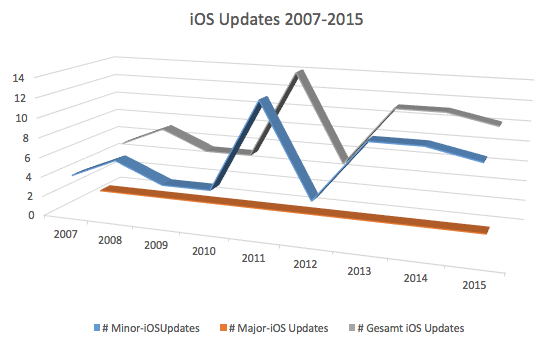
\includegraphics[scale=0.7]{Bilder/iOSUpdates}
        \caption{iOS Software Updates\cite{Apple[7]}}
        	\label{fig:iOS Software Updates}
\end{figure}

% ------ Hardcoded newpage -------
\newpage
Die „Jailbreak-Community“ benötigt im Durchschnitt 36 Tage, um eine neue iOS Version zu „jailbreaken“. Die „Bugs“, die ein Jailbreak ausnützt, sind meistens in mehreren iOS Versionen vorhanden. Nicht alle „Bugs“ werden von Apple geschlossen, es gibt Jailbreaks, die mehrere Jahre funktionieren. Dies gilt vor allem für ältere iOS Versionen und iOS Devices.

\begin{figure}[!ht]
        \centering
                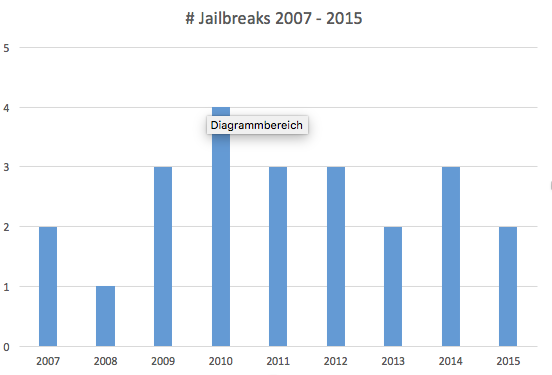
\includegraphics[scale=0.7]{Bilder/AnzahlJB}
        \caption{Anzahl iOS Jailbreak 2007 - 2015}
        	\label{fig:iOS Jailbreak}
\end{figure}


% ------------- Aufbau Jailbreak 9.x --------------------
\section{Aufbau Jailbreak iOS 9.x}
\label{sec:JBAufbau}
Damit ein Jailbreak auf einem iOS Device durchgeführt werden kann müssen Schritt für Schritt die iOS Sicherheitsschritte umgangen werden. Ab der iOS Version 8.1.3 sind für einen \glqq untethered Jailbreak\grqq{} fünf Schritte notwendig.

\begin{description}
\item[Dies sind die fünf iOS Sicherheitsmechanismen, die ein erfolgreicher Jailbreak umgehen muss]~\par
	\begin{enumerate}
	    \item Die Sandboxfunktionalität (siehe Kapitel: \ref{sec:Sandbox}) 
	     \item Das Signieren jedes Codes 
	    \item Erhalten der \glqq root\grqq{} Rechte
	    \item Das Patchen des Kernels
	  \end{enumerate}
\end{description} 

\cite{TaiG[1]}
\cite{TaiG[2]}
\cite{TaiG[3]}

% ------------- Jailbreak Step 1 --------------------
\subsection{Breaking out of the sandbox}
\label{sec:JBStep1}
Im ersten Schritt muss ein Bug im iOS und/oder einer Applikation gefunden werden, welcher es erlaubt \glqq die Sandbox\grqq{} (siehe Kapitel: \ref{sec:Sandbox}) zu umgehen. 

% ------------- Jailbreak Step 2 --------------------
\subsection{Obtaining arbitrary (unsigned) code execution}
\label{sec:JBStep2}

% ------------- Jailbreak Step 3 --------------------
\subsection{Obtaining root}
\label{sec:JBStep3}

% ------------- Jailbreak Step 4 --------------------
\subsection{Patching the Kernel}
\label{sec:JBStep4}
          % Jailbreak
%----------------------------------------------------------------
%
%  File    :  chapter4.tex
%
%  Authors :  Michael Fuska, FH Campus Wien, Austria
% 
%  Created :  08 Feb 2016
% 
%  Changed :  
% 
%----------------------------------------------------------------
\chapter{Mobile Apple Betriebssystem iOS}
\label{ch:iOS}
%------------------------------------------------------------------------------
%---------------------------------- iOS Grundlagen
\section{iOS Grundlagen}
\label{sec:iOSGrundlage}

Das mobile Apple Betriebsystem iOS basiert auf dem Desktop Betriebssystem des Mac OS X. Darwin ist ein frei erhältliches Linux basiertes Betriebssystem.Dieses Betriebssystem stellt die Grundlage für das Mac OS X dar. Der Kernel des Mac OS X ist der XNU-Kernel mit entsprechenden Adaptionen für das Mac OS X und dem mobilen Betriebssystem iOS.
\begin{figure}[htbp]
        \centering
                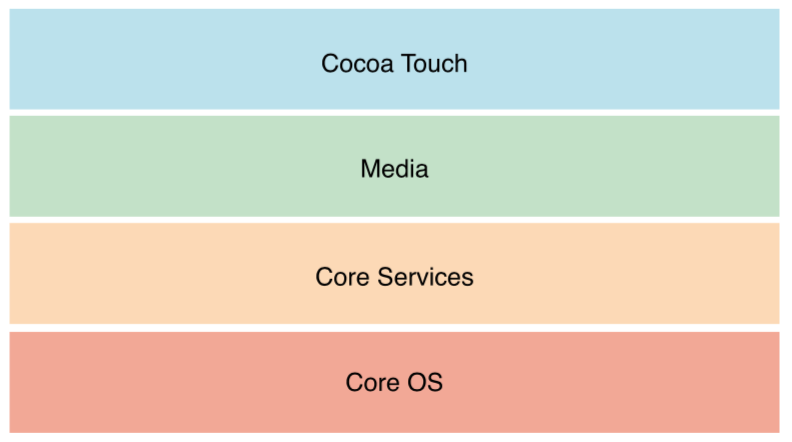
\includegraphics[height=5cm]{Bilder/Chapter3_SystemArchitektur}
        \caption{iOS Software Layer (\cite{Apple[6]}, S. XXXXXXXXX)}
        	\label{fig:iOS Software Layer}
\end{figure}
Die abgebildeten Schichten zeigen das abstrahiert iOS Betriebssystem. Der grösste Unterschied zwischen Mac OS X und iOS liegt im Cocoa Touch Layer.
  
\begin{description}
\item[Folgende \glqq Anforderungen\grqq{} werden an das iOS Software Layer Modell gestellt]~\par
	\begin{itemize}
		\item Sicherstellungen der \textbf{Datenintegrität}
		\item Gewährleistung der \textbf{Informationsvertraulichkeit}
		\item Sicherstellung der \textbf{User- und/oder Applikation Authentizität}
		\item Gewährleistung der \textbf{Daten/Informationsverbindlichkeit}
	\end{itemize}
\end{description}

%------------------------------------------------------------------------------
%---------------------------------- iOS Software Layer
\section{iOS Software Layer}
\label{sec:iOSSWLayer}

%---------------------------------- Core OS
\subsection{Core OS Layer}
\label{sec:CoreLayer}

Der \textbf{Core OS Layer} beinhaltet alle \textit{\glqq low-level Features\grqq{}} und auf diesen bauen alle anderen \textit{\glqq Frameworks\grqq{}} auf. iOS Applikationsentwickler kommen mit diesem Layer nur dann in Berührung, wenn sie sich mit der Sicherheit und mit Hardware-Kommunikation beschäftigen. 
\begin{description}
	\item[Core OS Layer Frameworks]~\par
	\begin{itemize}
		\item Accelerate Framework
		\item Core Bluetooth Framework
		\item External Accessory Framework
		\item Generic Security Service Framework
		\item Lost Authentication Framework
		\item Network Extension Framework
		\item Security Framework
		\item System
		\item 64-Bit Support
	\end{itemize}
\end{description}
 (vgl. \cite{Apple[6]}, S.49-52)
%---------------------------------- Core Service
\subsection{Core Service Layer}
\label{sec:CoreServiceLayer}		
Der \textbf{Core Service Layer} beinhaltet die fundamentalen System Services. Dieser Layer wird unterteilt in \textit{\glqq high-level Feature\grqq{}} und Core Services Frameworks.

\begin{description}
	\item[\textbf{High-level Feature dieses Layers}]~\par
	\begin{itemize}
		\item \textbf{Peer-to-Peer Services}
		\item \textbf{iCloud Storage}
		\item \textbf{Block Objects}
		\item \textbf{Data Protection}
		\item \textbf{File-Sharing Support}
		\item \textbf{Grand Central Dispatch}
		\item \textbf{In-App Purchase}
		\item \textbf{SQLite}
		\item \textbf{XML Support} 
	\end{itemize}
	
	\item[\textbf{Core Services Layer Frameworks}]~\par
	\begin{multicols}{2}
	\begin{itemize}
		\item Accounts Frameworks
		\item Address Book Framework
		\item Ad Support Framework
		\item CFNetwork Framework
		\item CloudKit Framework
		\item Core Data Framework
		\item Core Foundation Framework
		\item Core Location Framework
		\item Core Media Framework
		\item Core Motion Framework
		\item Core Telephony Framework
		\item EvenKit Framework
		\item Foundation Framework
		\item HealthKit Framework
		\item HomeKit Framework
		\item JavaScript Framework
		\item Mobile Core Services Framework
		\item Multipeer Connectivity Framework
		\item NewStandKit Framework
		\item PassKit Framework
		\item Quick Look Framework
		\item Safari Services Framework
		\item Social Framework
		\item StoreKit Framework
		\item System Configuration Framework
		\item WebKit Framework
	\end{itemize}
	\end{multicols}
\end{description}

(vgl. \cite{Apple[6]}, S.36-48)
%---------------------------------- Media Layer
\subsection{Media Layer}
\label{sec:MediaLayer}		
In diesem Layer sind alle Technologien zur Darstellung von Grafik, Video und das abspielen von Sound enthalten. Dieser Layer ist verantwortlich für das Design und den Sound der iOS Applikationen. 

\begin{description}
	\item[Dieser Layer stellt folgende Technologien zur Verfügung]~\par
    \begin{itemize}
		\item \textbf{Graphics Technologies}
		\item \textbf{Audio Technologies}
		\item \textbf{Video Technologies}
		\item \textbf{AirPlay}
    \end{itemize}

	\item[Media Layer Frameworks]~\par
	\begin{multicols}{2}
	\begin{itemize}
		\item Assets Library Framework
		\item AV Foundation Framework
		\item AVKit Framework
		\item CoreAudioKit Framework
		\item Core Graphics Framework
		\item Core Image Framework
		\item Core Text Framework
		\item Core Video Framework
		\item Game Controller Framework
		\item GLKit Framework
		\item Image I/O Framework
		\item Media Accessibility Framework
		\item Media Player Framework
		\item Metal Framework
		\item OpenGL ES Framework
		\item Photos Framework
		\item Photos UI Framework
		\item Quartz Core Framework
		\item SceneKit Framework
		\item SpriteKit Framework
         \end{itemize}
	\end{multicols}
\end{description}
(vgl. \cite{Apple[6]}, S.23-35)
%---------------------------------- Cocoa Touch Layer
\subsection{Cocoa Touch Layer}
\label{sec:CocoaTouchLayer}
Enthält die wichtigsten Frameworks um iOS Applikationen zu entwickeln. Dieser
Layer stellt die Basis Applikation Infrastruktur und folgende Key Technologien zur Verfügung

	\begin{itemize}
		\item \textbf{Multitasking}
		\item \textbf{Touch-based Input}
		\item \textbf{Push Notification}
		\item \textbf{High-level System Service}	
	\end{itemize}

\begin{description}
\item[Folgende Features sind in diesem Layer enthalten]~\par
	\begin{multicols}{2}
	\begin{itemize}
		\item App Extentision
		\item Handoff
		\item Document Picker
		\item AirDrop
		\item TextKit
		\item UIKit Dynamics
		\item Multitasking
		\item Auto Layout
		\item Storyboards
		\item UI State Preservation
		\item Apple Push Notification Service
		\item Local Notifications
		\item Gesture Recognizers
		\item Standard System View Controllers
         \end{itemize}
	\end{multicols}
	
	\item[Cocoa Touch Layer Frameworks]~\par
	\begin{multicols}{2}
	\begin{itemize}
		\item Address Book UI Framework
		\item EventKit UI Framework
		\item GameKit Framework
		\item iAd Framework
		\item MapKit Framework
		\item Message UI Framework
		\item Notification Center Framework
		\item PushKit Framework
		\item Twitter Framework
		\item UIKit Framework
         \end{itemize}
	\end{multicols}
\end{description}
(vgl. \cite{Apple[6]}, S.12-22)

%---------------------------------- iOS Device Security Architektur
\pagebreak
\section{iOS Device Security Architektur}
\label{sec:iOSSecArchitektur}

Der Sicherheitsmechanismus der iOS Device unterteilt sich in zwei Ebenen. 
\begin{figure}[htb]
  \begin{minipage}{0.6\textwidth} 
  		\begin{description}
   			\item[ iOS Sicherheitsebenen]~\par
         		\begin{enumerate}	
				\item  \textbf{iOS Software}
					\begin{enumerate}
       						\item File System
         					\item OS Partition
						\item User Partition (verschlüsselt)
						\item App Sandbox
						\item Data Protection Class
      					\end{enumerate}
      				\item  \textbf{iOS Hardware und Firmware}~\par
					\begin{enumerate}
       						\item Kernel
						\begin{enumerate}
						\item Secure Enclave
						\item Secure Element
         					\end{enumerate}	
						\item Crypto Engine
						\item Device Key
						\item Group Key
						\item Apple Root Certificate
      					\end{enumerate}
			\end{enumerate}
   		\end{description}
Die iOS Sicherheit passiert auf einer Kombination von Software, Hardware und Service um ein maximum an Sicherheit zu erreichen. (vgl. \cite{Apple[4]}, S.4)
	\end{minipage}
	\hfil
	\begin{minipage}{0.4\textwidth}
		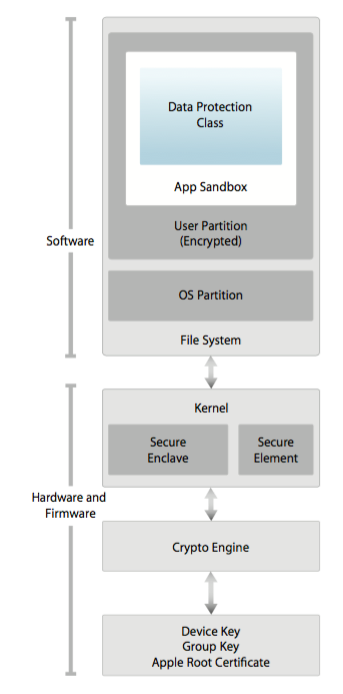
\includegraphics[width=\textwidth]{Bilder/Chapter3_SecArchitektur}
		\caption {iOS Security Architektur (\cite{Apple[4]}, S.4)}
        \label{fig:iOS Security Architektur}
	\end{minipage}
\end{figure}
		    	
%---------------------------- System Security
\subsection{System Security}
\label{sec:SystemSec}
Die \textbf{System Security} von iOS Device ist so kon­zep­ti­o­nie­rt, dass die Software und Hardware sicher über alle Kernkomponenten des Devices ist. Dies beinhaltet den sicheren Boot Prozess (Siehe Kapitel: \ref{sec:SecBootChain}), die Software Updates und die \textit{\glqq Secure Enclave \grqq{}} (Siehe Kapitel: \ref{sec:HardwareSecProtection}). Alle diese Maßnahmen dienen dazu, sicherzustellen, dass nur vertrauenswürdige Applikationen auf dem iOS Device ausgeführt werden können.\par 

Die enge Verbindung zwischen Hardware und Software eines iOS Geräte gewährleistet, dass alle Komponenten des Systems vertrauenswürdig sind, sowohl die Software als auch die Hardware. (vgl. \cite{Apple[4]}, S.5)
\begin{description}
\item[Apple führt unter dem Kapitel System Security folgende Features an]~\par
	%\begin{multicols}{2}
	\begin{itemize}
		\item Secure Boot Chain (siehe Kapitel:\ref{sec:SecBootChain})
 		\item System Software Authorization (siehe Kapitel:\ref{sec:SigningProcess})
 		\item Secure Enclave (Siehe Kapitel: \ref{sec:HardwareSecProtection})
 		\item Touch ID (Siehe Kapitel: \ref{sec:Passcode})
        \end{itemize}
	%\end{multicols}
\end{description}
(vgl. \cite{Apple[4]}, S.5-9)

%--------------------------- Encryption und Daten Sicherheit
\subsection{Encryption und Daten Sicherheit}
\label{sec:DataEnc}

Das iOS unterstützt standardmäßig eine Verschlüsselung und verschiedenste Datenschutzfunktionen für persönliche Daten und Unternehmensdaten. Die Sicherheitsinfrastruktur des iOS Devices ist so aufgebaut, dass selbst, wenn ein Teil des Betriebsystem kompromittiert ist, die anderen Bereiche des Devices, weiterhin sicher vor unerlaubten Zugriff sind. \par
Dies ist besonders für Unternehmen wichtig, da dadurch gewährleistet wird, dass vertrauliche Unternehmensdaten nicht gelesen werden können. Weitere iOS Features stellen sicher, dass selbst bei Diebstahl oder Verlust des iOS Devices die Daten sicher sind. Alle diese Features sind in der Standardkonfiguration aktiv gesetzt.


\begin{description}
\item[\parbox{\textwidth} {Apple führt unter dem Kapitel Encryption und Daten Sicherheit folgende Features an}]~\par
	\begin{itemize}
		\item \textbf{Hardware Security Features} (Siehe Kapitel: \ref{sec:HardwareSecProtection})
 		\item \textbf{File Data Protection} (Siehe Kapitel: \ref{sec:FileDataProtection})
 		\item \textbf{Passcodes} (Siehe Kapitel: \ref{sec:Passcode})
 		\item \textbf{Data Protection Classes}  (Siehe Kapitel: \ref{sec:HardwareSecProtection})
		\item \textbf{Keychain Data Protection} (Siehe Kapitel: \ref{sec:HardwareSecProtection})
	\end{itemize}
\end{description}
(vgl. \cite{Apple[4]}, S.10-17)

%------------------------------ Applikation Security
\subsection{Applikation Security}
\label{sec:AppSec}
Die Applikationen beinhalten das größte Sicherheitsrisiko für Betriebssysteme. Das Verhalten des Betriebssystems kann eine Applikationen negativ beeinflusst werden. Es kann die Sicherheit und die Verfügbarkeit des iOS Devices negativ beeinträchtigen. Des weiter kann die Integrität des Benutzerdaten durch unsicher Applikationen gefährdet werden.
\begin{description}
\item[\parbox{\textwidth} {Apple führt unter dem Kapitel Applikation Security folgende Features an}]~\par
	\begin{itemize}
		\item \textbf{App Code signing} (Siehe Kapitel: \ref{sec:SigningProcess}) 
		\item \textbf{Runtime process security} (Siehe Kapitel: \ref{sec:MemoryProtection})
		\item \textbf{Extensions}
		\item \textbf{App Groups} (Siehe Kapitel: \ref{sec:Sandbox})
		\item \textbf{Data Protection in Apps} (Siehe Kapitel: \ref{sec:SystemSec})

        \end{itemize}
\end{description}
(vgl. \cite{Apple[4]}, S.18-26)

%------------------------------ Network Security
\subsection{Network Security}
\label{sec:NetworkSec}
Die \textbf{ Netzwerk Sicherheit} ist ein wichtiger Bestandteil des Sicherheitskonzept und ergänzt die integrierten iOS Sicherheitsmechanismen. Die integrierten Sicherheitsmechanismen des mobilen Betriebssystem von Apple dienen dazu, die Daten auf dem Device zu schützen. Die Anforderungen an ein mobiles Device haben sich in den letzten Jahren dahin gehend verändert, dass der Zugriff auf externe Daten geschützt vorgenommen werden kann. Dieser Zugriff muss so abgesichert sein, dass die Datenübertragung sicher ist und die Usability des Produktes nicht eingeschränkt ist. Es werden Netzwerksicherheit Protokolle und Architekturen für eine authentifizierte, autorisierte und verschlüsselte Kommunikation verwendet.
\begin{description}
\item[\parbox{\textwidth} {Ein iOS Device verfügt über folgende Netzwerksicherheit Protokolle und Architekturen
an}]~\par
	\begin{itemize}
		\item \textbf{Virtual Private Network (VPN)}
 		\item \textbf{Single Sign-on}
 		\item \textbf{Internet Protocol Security (IPsec)}
 		\item \textbf{Transport Layer Security (TLS)} %(siehe Kapitel:\ref{sec:TLS})
		\item \textbf{Datagram Transport Layer Security (DTLS)}
        \end{itemize}
\end{description}
Des weiter werden die neuersten Standards für WLAN, Bluetooth und Mobilfunk-Verbindungen verwendet. (vgl. \cite{Apple[4]}, S.27-30)

%------------------------------ Apple Pay ----------------------------------
\subsection{Apple Pay}
\label{sec:ApplePay}

\textbf{Apple Pay} ist das interne Apple Zahlungssystem für mobile Geräte. Die Kommunikation findet über NFC statt. Neben NFC ist die App \textit{\glqq Wallet\grqq{}} Teil des Apple Pay Produkt.

\begin{description}
\item[\parbox{\textwidth} {Folgende Komponenten gehören zu dem Apple Pay Produkt}]~\par
	\begin{itemize}
		\item \textbf{Secure Element:} \\
        Alle Secure Element erfüllen den Industriestandard. Der zertifizierte Chip wird ein einer Java Card Plattform ausgeführt. Diese Elemente erfüllen den finanzindustrie Standard. 
 		\item \textbf{Near Field Communication (NFC) Controller:} \\
        Der NFC Controller und die NFC Kommunikation Protokolle sind für die Kommunikation zwischen den Anwendungsprozessoren und Secure Elementen zuständig.
 		\item \textbf{Wallet:} \\
        Die Wallet App ist für die Verwaltung der Kreditkarten und Debitkarten verantwortlich. 
            \begin{description}
                \item[\parbox{\textwidth} {Diese App ermöglicht es dem User}]~\par
                \begin{itemize}
                    \item die Kartendaten,
                    \item den Kartenaussteller,
                    \item die durchgeführten Transaktionen der einzelnen Karten und
                    \item vieles mehr
                \end{itemize}
            \end{description} 
        \textbf{abzuspeichern und anzuzeigen.}
        
 		\item \textbf{Secure Enclave:}\\
        Die Secure Enclave ist für den Authentifizierungsprozess einer Finanztransaktion zuständig. Des weiter werden in der Secure Enclave die Touch-ID Fingerabdrücke gespeichert.	
        \end{itemize}
\end{description}
(vgl. \cite{Apple[4]}, S.31-37)

%------------------------------ Internet services
\subsection{Internet Services}
\label{sec:InternetServices}

Apple hat sich die Prämisse gestellt stabile Applikationen mit guter Benutzbarkeit für den Benutzer zu entwickeln. 
\begin{description}
    \item[\parbox{\textwidth} {Beispiele für solche internen iOS Apps sind }]~\par
    \begin{itemize}
       \item iMessage,
       \item Facetime,
       \item iCloud und 
       \item iCloud Keychain.
    \end{itemize}
\end{description} 

Apple stellt den Entwicklern von Internet Diensten die Frameworks zur Verfügung, die auch für interne Apple Apps verwendet werden. Natürlich gelten für Internet Dienste die selben Sicherheitsziele, wie für die internen Apple Produkte. Diese Ziele beinhalten den \textit{\glqq sicheren Umgang mit den persönlichen Daten der Benutzer\grqq{}}, sowie \textit{\glqq den Schutz vor nicht autorisierten Zugriff auf die persönlichen Daten des Benutzers\grqq{}} und \textit{\glqq anderer Dienstleistungen\grqq{}}. Jeder Dienst verwendet eine eigene leistungsstarke Sicherheitsarchitektur ohne die Benutzerfreundlichkeit des gesamten iOS Devices zu beeinträchtigen. (vgl. \cite{Apple[4]}, S.38-49)

\begin{description}
    \item[\parbox{\textwidth} {Dies sind die Mainfeatures des Apple Internet Service}]~
    \begin{itemize}
        
        \item \textbf{Apple-ID:}\\
        Die \textbf{Apple-ID} ist Teil des persönliche Apple-Accounts, der zusammen mit dem \textit{\glqq Password\grqq{}} den Zugriff auf die Apple Service ermöglicht. 
        
        \item \textbf{iCloud:} \\
        Die \textbf{iCloud} ist der Apple Online-Dienst zum speichern und synchronisieren von Daten/Konfigurationen. 
        
        \item \textbf{iCloud Keychain:}\\
        Die \textbf{iCloud Keychain} ist das Apple Online \textit{\glqq Password Management System\grqq{}}. \begin{description}
                \item[\parbox{\textwidth} {Das Password Management System dient zum Speichern von}]~\par
                    \begin{itemize}
                        \item systemübergreifenden Passwörtern,
                        \item Login Daten,
                        \item WLAN-Zugangsdaten und 
                        \item Kreditkartendaten.
                    \end{itemize}
                \end{description} 
 
        \item \textbf{Continuity:}\\
        Darunter versteht Apple, dass Verteilen von Informationen und Services über mehrere iOS Devices. 
        \begin{description}
        \item[\parbox{\textwidth} {Beispiele für Continuity sind}]~\par
            \begin{itemize}
                \item Die Anrufannahme auf unterschiedlichen iOS Devices
                \item Die Möglichkeit Nachrichten auf unterschiedlichen iOS Devices zu lesen und zuschreiben.
                \item Das Verteilen von Dateien auf iOS Devices.
            \end{itemize}
        \end{description}  
    \end{itemize}
\end{description}

%------------------------------ Device Controls
\subsection{Device Controls}
\label{sec:DeviceControl}

Der \textbf{Device Control} Mechanismus von Apple hat die Aufgabe flexible Sicherheitsrichtlinien und Konfigurationen umzusetzen. Eine weitere Rahmenbedingung ist, dass die Konfiguration der Geräte leicht umsetzbar und verwaltbar ist.\par 
 Für Unternehmen bringt dies den Vorteil mit sich, dass Sicherheitsrichtlinien und Konfigurationen auf mehrere iOS Geräte verteilt werden können. Dadurch können Firmen sicherstellen, dass alle Geräte die selben Einstellungen besitzen. Des weiter ermöglicht es Mitarbeiter ihre eigenen Geräte im Unternehmen zu verwenden (BYOD). 

\begin{description}
    \item[\parbox{\textwidth} {Dies sind die Mainfeature des Apple Device Control Service} ]~\par
    \begin{multicols}{2}
    \begin{itemize}
        \item Passcode Sicherheit
        \item iOS pairing model
        \item Konfigurationsverteilung
        \item Mobile Device Management(MDM)
        \item Device Enrollment Program
        \item Device restriction
        \item Apple Configurator
        \item Supervised-only restrictions
        \item Remote wipe
        \item Find My iPhone and 
        \item Activation Lock
    \end{itemize}
    \end{multicols}
\end{description}
(vgl. \cite{Apple[4]}, S.50-55)
%----------------------------- Privacy Controls

\subsection{Datenschutzkontrolle}
\label{sec:PrivacyControls}
Das mobile Betriebssystem von Apple verfügt über zahlreiche integrierte Steuerelemente und Optionen. Diese iOS Einstellungen ermöglichen es dem Benutzer zu entscheiden, wie mit seinen persönlichen Daten umgegangen werden soll. Dies inkludiert welche App Zugriff auf welche Informationen bekommen soll. 

\begin{description}
    \item[\parbox{\textwidth} {Folgende Daten werden für die Ortung des Users verwendet (Location Service) }]~\par
    \begin{itemize}
        \item GPS Daten,
        \item Bluetooth Daten,
        \item öffentliche WLAN-Hotspots
        \item Mobilfunkmasten
    \end{itemize}
    Der User hat die Möglichkeit mit Hilfe von iOS Einstellungen zu definieren, welche App welche Location Daten verwenden kann.
    \item[\parbox{\textwidth} {Zu den persönlichen User-Daten zählen}]~\par
    \begin{multicols}{2}
    \begin{itemize}
        \item Kontakte
        \item Kalender
        \item Erinnerungen
        \item Fotos
        \item Aktivitätsdaten
        \item Accounts sozialer Netzwerke
        \item Mikrofon
        \item Kamera
        \item Bluetooth-Freigabe
    \end{itemize}
      \end{multicols}
\end{description}
(vgl. (\cite{Apple[4]}, S.56), (\cite{Apple[8]}, S.49))          % iOS Grundlagen
%----------------------------------------------------------------
%
%  File    :  chapter5.tex
%
%  Authors :  Michael Fuska, FH Campus Wien, Austria
% 
%  Created :  08 Feb 2016
% 
%  Changed :  
% 
%----------------------------------------------------------------
\chapter{iOS Sicherheitskonzepte}
\label{ch:iOSSicherheitsKonzepte}

%------------------------------------------------------------------------------
%------------------------------ Reduziertes Betriebsystem
\section{Reduziertes Betriebssystem}
\label{sec:reduziertesOS}
Unter iOS wurden die Angriffsvektoren für Hacker reduziert, indem das mobile Betriebssystem reduziert wurde. Der User hat nicht die Möglichkeit, auf den internen Flash Speicher des Gerätes zuzugreifen. Weder über einen File-Explorer noch über ein Terminalprogramm. 
\begin{description}
    \item[\parbox{\textwidth} {Unter anderem sind folgende Terminalprogramme unter iOS nicht verfügbar}]~\par
    \begin{itemize}
       \item telnet
       \item ssh
    \end{itemize}
\end{description} 
Auf einen Device mit Jailbreak können beide Terminalprogramme und verschiedenste File-Explorer installiert werden. Somit kann der User die Daten des iOS Device verwalten (lesen, schreiben, löschen und ändern).
\begin{description}
    \item[\parbox{\textwidth} {Aus Sicherheitsgründen sind folgende Dienste/Entwicklungsumgebungen auf einem iOS Device nicht installiert}]~\par
    \begin{itemize}
       \item Java
       \item Shell Programme (bash, sh, csh, usw.)
       \item Adobe Flash
    \end{itemize}
\end{description} 

%------------------------------------------------------------------------------
%------------------------------  Memory Protection
\section{Memory Protection Mechanism}
\label{sec:MemoryProtection}
Die wichtigsten \textbf{Memory Protection Mechanismen} unter iOS sind
\begin{enumerate}
    \item \textbf{Secure Boot Chain}
    \item \textbf{Address Space Layout Randomization (ASLR)}
    \item \textbf{Mandatory Access Control (MAC)}
\end{enumerate}

% -------------------------
%------------------------------ Secure boot chain
\subsection{Secure Boot Chain}
\label{sec:SecBootChain}

Die \textbf{Secure Boot Chain} ist eine Kernsicherheit-Funktionalität des iOSs. Jede Phase des Boot-Prozesses ist verschlüsselt. Jede Phase enthält den Key zum Entschlüsseln der nächsten Phase. Dadurch ist sichergestellt, dass die Boot Kette nicht unterbrochen wird. \par

Der \textit{\glqq Boot Read Only Memory (ROM)\grqq{}} ist der \textit{\glqq Root of Trust\grqq{}} der Secure Boot Chain. Im ersten Step wird das \textit{\glqq Root Zertifikat\grqq{}} aus dem ROM gelesen. Das Root Zertifikat wurde durch die \textit{\glqq Apple Certificate Authority (CA)\grqq{}} signiert. Der öffentliche Schlüssel des Root Zertifikates wird verwendet, um die Signatur des Low Level Boot Loaders zu prüfen. Wenn die Signatur erfolgreich validiert wurde, wird der LLB mit dem Key aus dem ROM entschlüsselt und geladen. Diese Schritte werden für jedes Modul/Phase des Secure Boot Chain durchgeführt. Diese Vorgangsweise  wird Secure Boot Chain genannt.

\begin{description}
    \item[\parbox{\textwidth}{Die Secure Boot Chain beinhaltet folgende Module/Phasen}]~\par
   \begin{enumerate}
        \item \textbf{Low Level Bootloader (LLB)},
        \item \textbf{iBoot},
        \item \textbf{Kernel},
        \item \textbf{Kernel Extension}
        \item \textbf{Baseband Firmware}.
    \end{enumerate}
\end{description} 

Die Secure Boot Chain stellt sicher, dass keine Veränderung der Hardware und/oder des iOS Kernels während des Boot Prozesses vorgenommen werden kann. Nach erfolgreicher Verifikation der Kernel Signatur, wird der Kernel entschlüsselt und das mobile Betriebsystem von Apple wird geladen. Im nächsten Schritt wird die Signatur jedes Prozesses, sowohl vom Betriebssystem als auch von den User Applikationen, validiert. Nur wenn die Prüfung der Signatur erfolgreich war, werden der Code und die Libraries in den Memory des iOS Devices geladen. Dies stellt sicher, dass nur eine Software auf einem iOS Gerät geladen werden kann, welche mit einem gültigen Zertifikat signiert wurde. (Vgl. \cite{Apple[4], Apple[5], Apple[6]})

% -------------------------
% -------------------------
%\subsection{Boot ROM}
%\label{sec:BootROM}
%% http://resources.infosecinstitute.com/understanding-ios-security-part-1/
%
%% -------------------------
%% -------------------------
%\subsection{Low Level Boot Loader}
%\label{sec:LowLevelBootLoader}
%
%% -------------------------
%% -------------------------
%\subsection{iBoot}
%\label{sec:iBoot}
%
%% -------------------------
%% -------------------------
%\subsection{Kernel}
%\label{sec:Kernel}
%
%------------------------------------------------------------------------------
%------------------------------ Secure Recovery Boot Chain
%\section{Secure Recovery Boot Chain}
%\label{sec:SecureRecoveryBootChain}

%\subsection{Recovery Mode}
%\label{sec:RecoveryMode}

% -------------------------
% -------------------------
\subsection{Address Space Layout Randomization (ASLR)}
\label{sec:ASLR}

Durch die Implementierung von \textbf{Address Space Layout Randomization (ASLR)} wurde die Exploitation von Softwarebugs unter iOS erheblich schwerer. ASLR hat die Aufgabe, beim Starten des Betriebssystems und der Programme diesen randomisierte Memory Adressen zuzuweisen. Dadurch ist die Zuweisung der Speicheradressen nicht mehr deterministisch. Wenn ASLR im vollen Funktionsumfang implementiert worden ist, muss ein Hacker mehrere Softwarefehler finden, um einen Memory Exploitation ausnützen zu können. Betriebssysteme, die ASLR nur teilweise implementiert haben, ermöglichen es Hackern, Memory Bereiche zu lokalisieren bzw. vorherzusagen, die \textit{\glqq writable\grqq{}} oder \textit{\glqq executable\grqq{}} sind, und somit können diese Systeme leichter angegriffen werden. (Vgl. \cite{Apple[4], ASLR[1], ASLR[2], ASLR[3], ASLR[4]})	 \par

Das mobile Betriebssystem von Apple unterstützt ASLR seit der iOS Version 4.3. Jede App hat die Möglichkeit, diesen Mechanismus mit dem Compiler Flag \textbf{Position Independent Executables (PIE)} zu aktivieren. Wenn die App mit dem PIE Flag kompiliert wurde, dann werdem
\begin{itemize}
    \item \textbf{dem Base Pointer(EBP),}
    \item \textbf{dem Textsegment,} 
    \item \textbf{dem Datensegment,}
    \item \textbf{dem BSS Segment,} 
    \item \textbf{dem Stack Segment,}
    \item \textbf{dem Heapsegment}
    \item \textbf{und den Libraries der App}
\end{itemize}
unterschiedliche \textit{\glqq virtual Memory-Adressen\grqq{}} zugewiesen. Alle unter iOS vorinstallierten Apps wurden mit diesem PIE Flag kompiliert. 

Die nachfolgenden Tabellen \ref{tab:PIE executable segment}, \ref{tab:PIE data segment}, \ref{tab:PIE stack segment}, \ref{tab:PIE heap segment}, \ref{tab:PIE libraries} und \ref{tab:PIE linker } zeigen die PIE Variationen

 \begin{table}
    \begin{center}
         \begin{tabular}{|p{6cm}|p{9cm}|} \hline
            Compiling Option PIE ist gesetzt & Code Segment \\ \hline
            Nein & fixe Memory Adresse\\ \hline
            Ja & randomisierte Memory Adresse per Ausführung (execution)\\ \hline
        \end{tabular}
        \caption{PIE executable segment (Vgl. \cite{iOSSec[5]}) }
       \label{tab:PIE executable segment}
    \end{center}
\end{table}

 \begin{table}
    \begin{center}
       \begin{tabular}{|p{6cm}|p{9cm}|} \hline
            Compiling Option PIE ist gesetzt & data segment\\ \hline
            Nein & fixe Memory Adresse\\ \hline
            Ja & randomisierte Memory Adresse per Ausführung (execution)\\ \hline
        \end{tabular}
        \caption{PIE data segment (Vgl. \cite{iOSSec[5]})}
       \label{tab:PIE data segment}
    \end{center}
\end{table}

\begin{table}
    \begin{center}
        \begin{tabular}{|p{6cm}|p{9cm}|} \hline
            Compiling Option PIE ist gesetzt & Stack Segment\\ \hline
            Nein & fixe Memory Adresse\\ \hline
             Ja & randomisierte Memory Adresse per Ausführung (execution)\\ \hline
        \end{tabular}
         \caption{PIE stack segment (Vgl. \cite{iOSSec[5]})}
       \label{tab:PIE stack segment}
    \end{center}
\end{table}    

\begin{table}
    \begin{center}
       \begin{tabular}{|p{6cm}|p{9cm}|} \hline
            Compiling Option PIE ist gesetzt & Heap Segment\\ \hline
            Nein & randomisierte Memory Adresse per Ausführung (execution)\\ \hline
            Ja & randomisierte Memory Adresse per Ausführung (execution)\\ \hline
        \end{tabular}
        \caption{PIE heap segment (Vgl. \cite{iOSSec[5]}) }
       \label{tab:PIE heap segment}
    \end{center}
\end{table}

\begin{table}
    \begin{center}
      \begin{tabular}{|p{6cm}|p{9cm}|} \hline
            Compiling Option PIE ist gesetzt & Libraries \\ \hline
            Nein & randomisierte Memory Adresse per Device boot\\ \hline
            Ja & randomisierte Memory Adresse per Device boot \\ \hline
        \end{tabular}
        \caption{PIE libraries (Vgl. \cite{iOSSec[5]})}
       \label{tab:PIE libraries}
    \end{center}
\end{table}

 \begin{table}
    \begin{center}
        \begin{tabular}{|p{6cm}|p{9cm}|} \hline
            Compiling Option PIE ist gesetzt & Linker  \\ \hline
            Nein & fixe Memory Adresse\\ \hline
            Ja & randomisierte Memory Adresse per Ausführung (execution)\\ \hline
        \end{tabular}
        \caption{PIE linker (Vgl. \cite{iOSSec[5]})}
       \label{tab:PIE linker }
    \end{center}
\end{table}

% -------------------------
% -------------------------
\subsection{Mandatory Access Control}
\label{sec:MAC}

 \textbf{Mandatory Access Control (MAC)} ist ein Konzept zur Kontrolle und Steuerung von Zugriffsrechten. MAC überprüft jeden ausführbaren Code und jede Library, die in den Memory geladen werden sollen. Im Gegensatz dazu prüft \textbf{Data Execution Prevention (DEP)} nur Binaries. iOS erfährt somit einen deutlichen Sicherheitsgewinn gegenüber anderen mobilen Betriebssystemen. \par 
 MAC wurde mit der iOS Version 2.0 eingeführt. Bis zum heutigen Zeitpunkt gibt es keinen Weg, um diese Zugriffskontrolle zu umgehen. Von jedem ausführbaren Code und jeder Library wird die Signatur geprüft, bevor die Daten in den virtuellen Memory geladen werden. (Vgl. \cite{iOSSec[5], Hacking[1]})
Der MAC Mechanismus hat zwei Vorteile gegenüber anderen Memory Protection Systemen. \par 
Erstens, Malware kann auf einem iOS Gerät nur ausgeführt werden, wenn diese auch zuvor von einem gültigen Zertifikat signiert worden ist. Es gibt Beispiele, in denen es Hackern gelungen ist, die Malware in einer App so zu verstecken, dass die App offiziell von Apple signiert worden ist. Dies konnte erreicht werden, indem Malware in Code Branches versteckt wurde, die in dem normalen Codefluss der App nie durchlaufen wird. (Vgl. \cite{iOSSec[5], Hacking[1]}) \par
 Der zweite Vorteil ist, dass die Exploits nur unter Anwendung von \textit{ \glqq Return Oriented Programming(ROP)\grqq{} } durchgeführt werden können. ROP ist weitaus komplexer als normale Shell Code Exploits.(Vgl. \cite{Architecture[1], Architecture[2], Architecture[3], ROP[1], ROP[2], iOSSec[5], Hacking[1]})

MAC wurde unter iOS im \textbf{Mandatory Access Control Framework(MACF)} implementiert. Für iOS wurden zwei \textit{\glqq mandatory access control policies\grqq{}} konfiguriert
\begin{enumerate}
   \item Sandbox (Siehe Kapitel \ref{sec:Sandbox})
   \item AMFI (Siehe Kapitel \ref{sec:AMFI})
\end{enumerate}
(Vgl. \cite{iOSSec[5], Hacking[1]})

% -------------------------
% -------------------------
\subsubsection{Apple Mobile File Integrity (AMFI)}
\label{sec:AMFI}
\textbf{AMFI } ist eine Kernel Extension, die den Code Signing Sicherheitsmechanismus implementiert hat. Die \textbf{AMFI Kernel Extension} überprüft die Signatur von jedem ausführbaren Code und von jeder Library. Sollten die Signatur (CDHash) nicht durch die AMFI Kernel Extension validiert werden können, wird über ein \textit{\glqq Remote Procedure Call (RPC) Interface\grqq{}} (Userspace) versucht, den Prozess zu validieren. Folgende Programmschnittstellen (Hooks) stehen der AMFI Kernel Extension für die Validierung der Signatur zur Verfügung

\begin{itemize}
    \item \label{item:AMFIfunc} \textbf{mpo\_vnode\_check\_signature:} \\
    Dieser Funktion wird als Parameter der CDHash übergeben und es wird überprüft, ob der CDHash im \textbf{static} oder \textbf{dynamic trust cache} eingetragen ist. Wenn nicht, muss der CDHash über das RPC Interface validiert werden. (Siehe Kapitel: \ref{sec:SignediOSApp}) (Vgl. \cite{iOSSec[5], Hacking[1]})
    \item \textbf{mpo\_vnode\_check\_exec:}\\
    Diese Funktion setzt die Flags CS\_HARD und CS\_KILL in der \textit{\glqq proc-Struktur\grqq{}} des Prozesses. (Vgl.\cite{iOSSec[5],  Hacking[1]})
    \item \textbf{mpo\_proc\_check\_get\_task:}\\
    Diese Funktion prüft die Entitlements get-task-allow and task\_for\_pid-allow. Wenn beide gesetzt sind, hat der Prozess Zugriff auf den \textit{\glqq Task Control Port\grqq{}}. Damit erhält  die App Zugriff auf die Debug-Informationen des Systems. (Vgl. \cite{iOSSec[5],  Hacking[1]})
    
    \item \textbf{mpo\_proc\_check\_run\_cs\_invalid:} \\
    Mit diesem Hook kann definiert werden, ob ein Programm ausgeführt werden darf, auch wenn das System festgestellt hat, dass dieses Programm nicht vertrauenswürdig ist. Dieser Fall kann eintreten, wenn das Programm nicht überprüft werden konnte oder der Code verändert wurde. Hierfür müssen die Entitlements 
    \begin{itemize}
        \item get-task-allow, 
        \item run-invalid-allow 
        \item und run-unsigned-code 
     \end{itemize} 
     gesetzt sein. (Vgl. \cite{iOSSec[5]} S.5, \cite{Hacking[1]})
    
    \item \textbf{mpo\_proc\_check\_map\_anon:}\\
    Nur in dem Fall, wenn der Prozess das Dynamic Code Signing Entitlement gesetzt hat, kann der Prozess anonymous Memory allokieren. (Vgl. \cite{iOSSec[5],  Hacking[1]})
\end{itemize}

Die AMFI Kernel Extension setzt die \textit{\glqq csflags\grqq{}} in der \textit{\glqq proc-Struktur\grqq{}} jedes Prozesses. Bei der Allokation und der Verwaltung der virtuellen Memory Pages werden die csflags des Prozesses vom Kernel überprüft. Diese Funktionalität ist das Bindeglied zwischen der Signatur/Entitlements der App und der virtuellen Speicherverwaltung des iOS Devices. 

%Thus, the kernel knows whether the process is successfully validated or not. The Table \ref{tab:CSFLAGS} describes the possible values of the csflags that can be set by the amfi kernel extension. \cite{iOSSec[5], Hacking[1]}
Alle definierten \textit{\glqq csflags\grqq{}} werden in der Tabelle: \ref{tab:CSFLAGS} angeführt.
\begin{table}[ht]
\begin{center}
\begin{tabular}{|l|c|p{8cm}|} \hline
  Flag Name & Value & Beschreibung\\ \hline
CS\_VALID & 0x00001 & Der Prozess ist dynamisch \textit{\glqq valid\grqq{}} \\ \hline
CS\_HARD & 0x00100 & Der Prozess darf keine \textit{\glqq invalid Page\grqq{}} laden.\\ \hline
CS\_KILL & 0x00200 & Der Prozess sollte \textit{\glqq beendet\grqq{}} werden, wenn der Prozess dynamisch \textit{\glqq invalid\grqq{}} werden würde.\\ \hline
CS\_EXEC\_ SET\_HARD & 0x01000 & Der Prozess setzt das CS\_HARD Flag für jeden ausgeführten Childprozess.\\ \hline
CS\_EXEC\_ SET\_KILL & 0x02000 & Der Prozess setzt das CS\_KILL Flag für jeden ausgeführten Childprozess. \\ \hline
CS\_KILLED & 0x10000 & Der Process wurde vom Kernel \textit{\glqq beendet\grqq{}} bevor dieser dynamisch \textit{\glqq invalid\grqq{}} ist.\\ \hline
\end{tabular} 
\caption{Value \textit{\glqq csflags\grqq{}} (Vgl. \cite{iOSSec[5]} S.11)}
\label{tab:CSFLAGS}
\end{center}
\end{table}


\paragraph{Zusammenfassend:} Es gibt drei Möglichkeiten für die AMFI Kernel Extension, die Signatur(CDHash) einer App zu validieren
\begin{enumerate}
    \item \textbf{Static trusted cache:} \\
    In diesem permanenten Speicher werden alle CDHash gespeichert, die fixer Bestandteil des mobilen Betriebssystems von Apple sind.  
    \item \textbf{Dynamic trusted cache:} \\
    Dies ist ein dynamischer Speicher in dem alle CDHashes gespeichert werden, die schon einmal erfolgreich verifiziert wurden. Mit jedem Neustart des iOS Gerätes wird dieser Speicher neu initialisiert.
    \item \textbf{AMFI RPC Interface} 
\end{enumerate}   
  
 Aus sicherheitstechnischen Gründen wurde die Verifizierung des CDHash vom \textit{\glqq Kernelspace\grqq{}} in den \textit{\glqq Userspace\grqq{}} ausgelagert. Damit werden die sehr komplexen und teuren kryptographische Rechenoperationen nicht mehr im sicherheitskritischen Kernelspace durchgeführt. Die Kommunikation zwischen der AMFI Kernel Extension (Kernelspace) und dem \textit{\glqq amfid Dämon (Userspace)\grqq{}} findet über die Remote Prozedur Calls(RPC) statt. Für diese Interprozesskommunikation stehen zwei Prozeduren zur Verfügung. Diese werden im Table \ref{tab:AMFID} beschrieben. (Vgl. \cite{iOSSec[5]} S.13, \cite{Mach[1]}) 

\begin{table}[ht]
\begin{center}
\begin{tabular}{|c|p{8,5cm}|} \hline
  Funktion & Beschreibung\\ \hline
verify\_code\_directory &  
Diese Funktion überprüft den CDHash und die Signatur der App. Es wird die Gültigkeit und die Vertraulichkeit der Signatur überprüft. Die Grundlagen für diese Prüfung sind das Apple Zertifikat (ROM) und das mit der App installierte Provisioning Profiles.\\ \hline

permit\_unrestricted\_ debugging &  
Diese Funktion überprüft die UDIDs der Provisioning Profiles des iOSs. Die Provisioning Profiles wurden mit den Apps auf dem iOS Device installiert. Es wird geprüft, ob für die UDID ein uneingeschränktes Debugging erlaubt ist. \\ \hline
\end{tabular} 
\caption{AMFI Daemon Mach RPC Interface (Vgl. \cite{iOSSec[5]} S.13)}
\label{tab:AMFID}
\end{center}
\end{table}

% -------------------------
% -------------------------
\subsubsection{Virtual Memory Pages}
\label{sec:virMemoryPages}
 Als \textbf{virtual Memory} wird die Technik bezeichnet, die den \textit{\glqq Adressraum\grqq{}} eines Prozesses unabhängig vom physischen Arbeitsspeicher des iOS Devices macht. Der Begriff \textbf{Paging} bezeichnet die Abbildung der virtuellen Adressen auf die physischen.\par 
Unter iOS gibt es zwei verschiedene Typen von virtuellen Memory Pages, die sich in den gesetzten Permissions unterscheiden 

\begin{enumerate}
    \item Lese- (read) und Schreibzugriff (write)
    \item Lesezugriff (read) und ausführbarer Zugriff (execute)
\end{enumerate}
Diese Permissions verhindern, dass der Inhalt des Speichers nach dem Laden verändert werden kann. Ein weiterer Vorteil ist, dass das Erzeugen von \textit{\glqq neuen dynamischen Codes\grqq{}} unterbunden wird. iOS macht  nur für einige Apps/Prozesse eine Ausnahme von dieser Regel. Der \textit{\glqq MobileSafari Webbrowser\grqq}, ist einer dieser Apps und kann zur Laufzeit \textit{\glqq dynamische HTML Seiten\grqq{}} generieren (Java Script). (Just in Time(JIT) Kapitel: \ref{sec:Jit}).


%CSE is built into the iOS kernel’s virtual memory system and most of its implementation is visible in Apple’s open source xnu kernel7, which is shared between iOS and Mac OS X. In essence, the virtual memory system tracks the validity of executable memory Pages and the process as a whole using the “dirty” bit used to implement Copy-on-Write (COW) semantics and virtual memory Pages -ins. When an executable memory Pages is Pages d-in and is marked as being “dirty”, its signature may have been invalidated and it must be reverified. New executable memory Pages are always “dirty”. If a single memory Pages is found to be invalid, then the entire process’ code signing validity is also set to be invalid.
%The code signing validity of the process is tracked with the CS_VALID flag in the csflags member of the kernel’s proc structure for that process. If the executable’s code signing signature has been validated prior to it being executed, the process begins execution with the CS_VALID flag set. If the process becomes invalid, then this flag will be cleared. What happens next depends on the CS_KILL flag. If this flag is set, the kernel will forcibly kill the process once it becomes invalid. On Mac OS X, the default is to not set this flag so that processes created from signed binaries may become invalid. On iOS, however, this flag is set by default so the process is killed once it becomes invalid. The flags defined for this field and a system call (csops) for getting and setting them from user space are documented in bsd/sys/codesign.h. The defined flags are also summarized in the table below:

% -------------------------
% -------------------------
\subsubsection{Dynamisches Code Signing (DCS)}
\label{sec:Jit}

Mit der iOS Version 2.0 wurde \textbf{Dynamisches Code Signing (DCS)} eingeführt, um den Performance-Ansprüchen der User gerecht zu werden. Es wurden in den unterschiedlichen iOS Versionen immer wieder DCS-Bugs behoben, bis die endgültige DCS-Version in iOS Version 4.3 veröffentlicht wurde. 
\paragraph{Just In Time (JIT)} wird unter iOS mit Hilfe von DCS ermöglicht. Der JIT-Compiler übersetzt zur Laufzeit das Programm in Bytecode. Der Bytecode wird in einen bestimmten Speicher geschrieben und ausgeführt. Somit muss es auch unter iOS einen Speicherbereich im virtual Memory geben, der sowohl beschreibbar als auch ausführbar ist.  JIT ist aber aus Sicherheits- und Performance-Gründen auf einige wenige Anwendungen beschränkt. Weiter wird sichergestellt, dass immer nur ein Prozess Zugang zu einem schreib- und ausführbaren Memory Bereich hat. Nur Prozesse, die das Entitlement \textbf{dynamic-codesigning} (Siehe Abbildung: \ref{fig:JIT}) gesetzt haben, können JIT verwenden und diesen speziellen Speicherbereich anfordern. Dadurch kann JavaScript im MobileSafari Webbrowser verwendet werden. (Vgl. \cite{JIT[1], ASLR[4]})

Es werden für eine JIT Request immer 16MB an Speicher reserviert. Der Kernel setzt nach der Prüfung der Entitlement, der Signatur und der Prüfung, ob dieser Prozess JIT verwenden darf, die entsprechenden Berechtigungen(RWX) im Virtual Memory.

\begin{figure}[htp!]
        \centering
                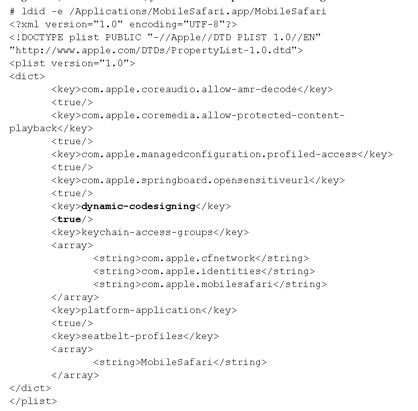
\includegraphics[scale=0.8]{JIT}
        \caption{Just in Time Entitlement (Vgl. \cite{Hacking[1]}) }
        \label{fig:JIT}
\end{figure}
% -------------------------
% -------------------------
\section{Signieren von Apps}
\label{sec:SigningProcess}

Apple führte mit der iOS Version 2.0 \textit{\glqq das verpflichtende Signieren von Apps\grqq{}} ein, um ausführbaren Codes und Libraries zur Laufzeit zu prüfen. Das Signieren einer App verhindert, dass 
\begin{itemize}
    \item \textbf{unsignierte Libraries,
}    \item \textbf{ein neuer Code zur Laufzeit,} 
    \item \textbf{und/oder ein selbstmodifizierender Code geladen und ausgeführt werden.}
\end{itemize}
Jede App wird mit einem Zertifikat signiert. Dadurch wird eine digitale Identität einer App zugeordnet. (Vgl. \cite{Cert[2], Cert[3]}).
\begin{description}
    \item[\parbox{\textwidth} {Eine App kann auf zwei Arten signiert werden}]~\par
   \begin{enumerate}
        \item Die Apps werden mit dem Apple Root-Zertifikat signiert und mit Hilfe von iTunes verteilt. 
        
        \item Apple autorisiert \textit{\glqq Third Parties\grqq}, dadurch können Unternehmen ihre Apps selbst signieren und verteilen. Die Verteilung der Apps kann dadurch in einem geschlossenen Userkreis stattfinden. Mit den Apps wird auch das entsprechende \textit{\glqq Provisioning Profile\grqq{}} (Siehe Kapitel: \ref{sec:ProvisioningProfile}) verteilt.
    \end{enumerate} 
\end{description} 
(Vgl. \cite{Sign[1], Sign[2], Sign[3], Sign[4], Sign[5], ROP[1]}) \par 
Die Signatur der App wird von der AMFI Kernel Extension (Siehe Kapitel: \ref{sec:AMFI}) geprüft, und es wird sichergestellt, dass nur ein valider Code vom Prozessor ausgeführt wird.    
 
 %------------------------------------------------------------------------- 
\subsection{Provisioning Profile}
\label{sec:ProvisioningProfile}
Das \textbf{Provisioning Profile} ist ein XML formatiertes File, in dem die \textit{\glqq Properties (Einstellungen)\grqq{}} der App gespeichert werden. Die Einstellungen werden in einem verschachtelten \textit{\glqq Schlüssel-Werte Paar (key-value pair)\grqq{}} abgelegt. Neben den unterschiedlichsten Konfigurationsmöglichkeiten und Entitlements enthält das Provisioning Profile auch das Developer Zertifikat(Public Key). Der Public Key wird zum Überprüfen der Signatur der App benötigt. (Vgl. \cite{iOSSec[5]} S.5, \cite{Hacking[1], ProvisioningProfile[1], ProvisioningProfile[2]}) \par
Ein wichtiger Bestandteil des Provisioning Profile ist das \textit{\glqq Entitlement Item\grqq{}}. Mit dem Entitlement Item legt der Entwickler die \textit{\glqq Permissions\grqq{}} für seine App fest. Weiter ist es möglich, die Unique Device Identifiers (UDIDs) im Provisioning Profile festzulegen, dies hat zur Folge, dass die App nur auf dem iOS Devices mit diesen UDIDs läuft. (Vgl. \cite{iOSSec[5]} S.5) \par 

\begin{description}
    \item[\parbox{\textwidth} {Es gibt drei unterschiedliche Arten von Provisioning Profiles }]~\par
    \begin{enumerate}
        \item \textbf{On-device Profile} \newline
Mit diesem Profile hat der Entwickler die Möglichkeit, seine Apps auf seinen Devices zu testen. Die Konfiguration des Provisioning Profile wird über das iOS Developer Portal durchgeführt. (Vgl. \cite{iOSSec[5]} S.5, \cite{AppDist[1]})
    
        \item \textbf{Ad-Hoc provisioning Profile} \newline
Dieses Profile gibt dem Entwickler die Möglichkeit, seine Apps auf bis zu 100 Devices zu installieren, somit sind erweiterte Applikationstests möglich. (Vgl. \cite{iOSSec[5]} S.5, \cite{AppDist[1]})
    
        \item \textbf{Enterprise provisioning Profile} \newline
Mit diesem Profile gibt es keine Einschränkungen, hinsichtlich der Anzahl der Devices. (Vgl. \cite{iOSSec[5]} S.5, \cite{AppDist[1]})
    \end{enumerate}
\end{description} 


Die Funktion \textit{\glqq MISProvisioningProfileCheckValidity\grqq{}} der Library \textit{\glqq /usr/lib/libmis.dylib\grqq{}} überprüft die Gültigkeit des Provisioning Profile.(Vgl. \cite{Cache[1]}) \par
 In der Systemeinstellung des iOS Devices werden alle auf dem Device installierten Provisioning Profile angezeigt. Nur wenn das Provisioning Profile gültig ist, kann das Profile am Gerät installiert und verwendet werden.(Vgl. \cite{iOSSec[5]} S.5, \cite{AppDist[1], Hacking[1]}) \par

\begin{description}
    \item[\parbox{\textwidth} {Stefan Esser beschreibt in seinem iOS Hacker's Handbook die Konditionen zur Überprüfung der Gültigkeit des Provisioning Profile wie folgt \cite{Hacking[1]} }]~\par
    \begin{itemize}
        \item \glqq \textit{The signing certificate must be issued by the Apple iPhone Certification Authority.}\grqq{} (Vgl. \cite{iOSSec[5]} S.5) 
    
        \item  \glqq \textit{The signing certificate must be named Apple iPhone OS Provisioning Profile Signing.}\grqq{} (Vgl. \cite{iOSSec[5]} S.5)
    
        \item  \glqq \textit{The certificate signing chain must be no longer than three links.}\grqq{} (\cite{Hacking[1]}, vgl. \cite{iOSSec[5]} S.5)     
    
        \item  \glqq \textit{The root certificate (referred to as the “Apple CA”) must have a particular SHA1 hash.}\grqq{} (Vgl. \cite{iOSSec[5]} S.5)    
    
        \item  \glqq \textit{The provisioning profile version number must be 1.}\grqq{} ((Vgl. \cite{iOSSec[5]} S.5)     
        \item  \glqq \textit{The provisioning profile must contain the UDID of this device or the profile must contain the key ProvisionsAllDevices.}\grqq{} (Vgl. \cite{iOSSec[5]} S.5)    
        \item  \glqq \textit{The profile must not expired.}\grqq{} (Vgl. \cite{iOSSec[5]} S.5) 
    \end{itemize}
\end{description} 

Mit den \glqq openssl\grqq{} (siehe Listing: \ref{list:secProP}) und \glqq security\grqq{} (siehe Listing: \ref{list:openProP}) Befehlen können die Items eines Provisioning Profile aufgelistet werden. Der \glqq openssl --verify\grqq{} Parameter ermöglicht es zusätzlich, das Profile zu verifizieren. 
\newline

\lstset{
    language=bash,
    }
\begin{lstlisting}[captionpos=b, caption={Befehl: security}, label=list:secProP]
security cms -D -i "filename" 
\end{lstlisting}

\begin{lstlisting}[captionpos=b, caption={Befehl: openssl -- (Siehe Abbildung: \ref{fig:ProvisioningProfile})}, label=list:openProP]
openssl smime -in filename -inform der -verify
\end{lstlisting}

\begin{figure}[htp!]
        \centering
                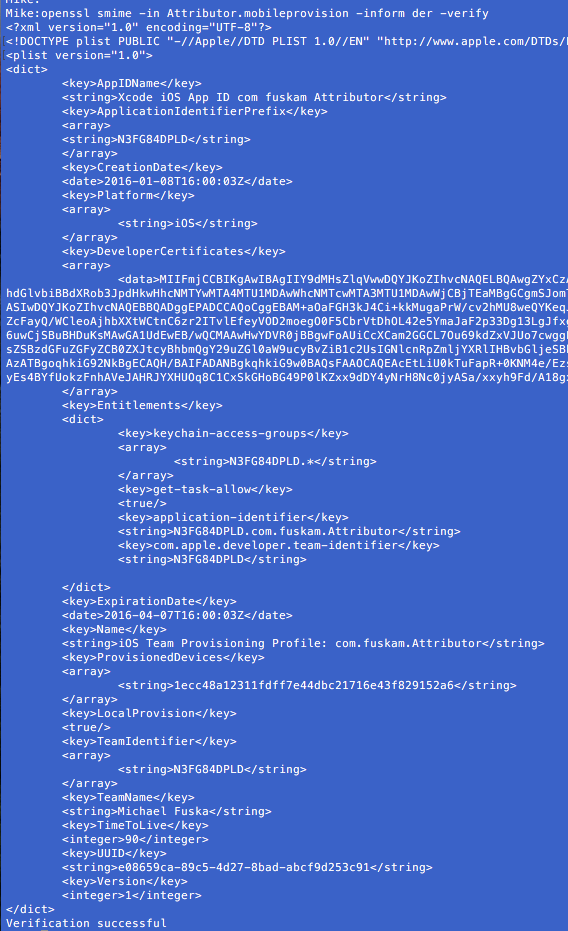
\includegraphics[scale=0.6]{SGML-Format}
        \caption{Provisioning Profile}
        \label{fig:ProvisioningProfile}
\end{figure}

\paragraph{Alle Items eines Provisioning Profile werden nachfolgend aufgelistet}
\begin{enumerate}
% --------APPIDNAME --------------
    \item AppIDName Item

\begin{lstlisting}[captionpos=b, caption={AppIDName Item}]
<key>AppIDName</key>
<string>Xcode iOS appID com fuskam Attributor</string>
\end{lstlisting}
Dieses Item beschreibt den Namen der App inklusive Namespace. (Vgl. \cite{iOSSec[5], Hacking[1]})

%-----------------APPLICATIONIDENTIFIERPREFIX ------------------
    \item ApplicationIdentifierPrefix Item
\begin{lstlisting}[captionpos=b, caption={ApplicationIdentifierPrefix Item}]
<key>ApplicationIdentifierPrefix</key>
<array>
    <string>N3FG84DPLD</string>
</array>
\end{lstlisting}
Dieses Item beschreibt den Namen der App im Provisioning Portal. Es ist ein zehn Zeichen langer String, welcher im Provisioning Portal generiert worden ist. Der ApplicationIdentifierPrefix wird immer dann erzeugt, wenn eine App ID generiert wird. Dieses Item ermöglicht es, Daten zwischen unterschiedlichen Apps zu verteilen. (Vgl. \cite{iOSSec[5], Hacking[1]})

%------CREATION DATE --------------
    \item CreationDate Item
\begin{lstlisting}[ captionpos=b, caption={CreationDate Item}]        
<key>CreationDate</key>
<date>2016-01-08T16:00:03Z</date>
\end{lstlisting}
Dieses Item beinhaltet den Zeitstempel der Provisioning Profile Generierung. (Vgl. \cite{iOSSec[5], Hacking[1]})

% ----------- PLATFORM --------------------
    \item Platform Item
\begin{lstlisting}[captionpos=b, caption={Platform Item}]        
<key>Platform</key>
<array>
    <string>iOS</string>
</array>
\end{lstlisting}
Dieser Item beinhaltet eine Betriebssystem Liste(Array). Auf diesen Systemen kann die App installiert und ausgeführt werden. (Vgl. \cite{iOSSec[5], Hacking[1]})

%------ DEVELOPERCERTIFICATES -----------------------
    \item DeveloperCertificates Item
\begin{lstlisting}[captionpos=b, caption={DeveloperCertificates Item}]        
<key>DeveloperCertificates</key>
<array                
    <data>..... </data>
</array>
\end{lstlisting}
Dieses Item beinhaltet eine Developer Zertifikat Liste(Array). Jedes Zertifikat ist \textit{\glqq base64\grqq{}} codiert. Mit dem \glqq openssl\grqq{} Befehl können alle Attribute des Zertifikats angezeigt werden. (Vgl. \cite{iOSSec[5], Hacking[1]}) \newline

\lstset{
    language=bash,
    }
\begin{lstlisting}[captionpos=b, caption={Befehl: openssl -- (Siehe Abbildung: \ref{fig:DeveloperCertificates})}]
openssl x509 -text -in Attributor.pem 
\end{lstlisting}

\begin{figure}[!ht]
        \centering
                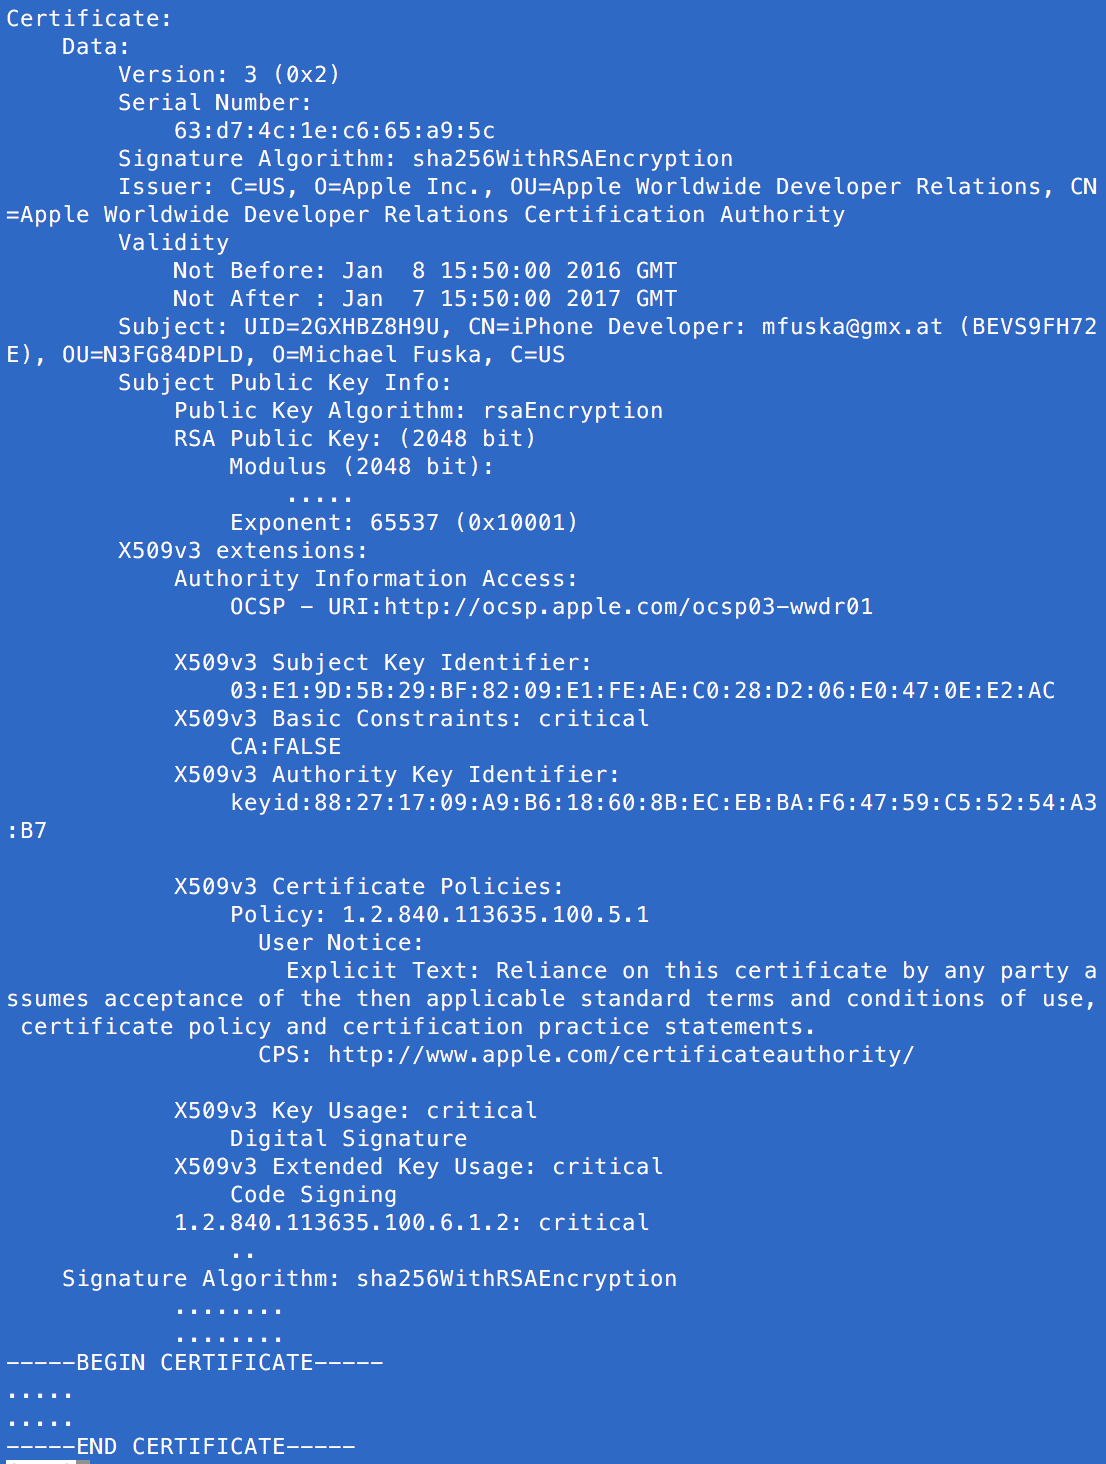
\includegraphics[scale=0.7]{Cert-output}
        \caption{Developer Certificates}
        \label{fig:DeveloperCertificates}
\end{figure}

%-------------ENTITLEMENTS -----------------------
    \item Entitlements Item
\begin{lstlisting}[captionpos=b, caption={Entitlements Item}]
<key>Entitlements</key>
<dict>
    <key>keychain-access-groups</key>
    <array>
        <string>N3FG84DPLD.*</string>           
    </array>
    <key>get-task-allow</key>
    <true/>
    <key>application-identifier</key>
    <string>N3FG84DPLD.com.fuskam.Attributor</string>
    <key>com.apple.developer.team-identifier</key>
    <string>N3FG84DPLD</string>
</dict>
\end{lstlisting}

Nachfolgend werden die möglichen \textit{\glqq Entitlements-Key\grqq{}} beschrieben:

\paragraph{keychain-access-groups:}
Dieses Entitlement verwaltet eine Liste (Array) von ApplicationIdentifierPrefix inklusive Namespace und ist ein Datensicherheit-Mechanismus für Apps. \par 
    \glqq \textit{This entitlement defines an array of strings corresponding to keychains you intend the app to have access to. Each string value in the array are of the format: <prefix>.<bundle\_id>. By default, Xcode creates this entitlement for you a value equal to the application-identifier entitlement. All prefixes in this array of strings must match.}\grqq{} (\cite{iOSSec[5]} S.8)

\paragraph{get-task-allow:} 
\glqq\textit{This entitlement permits applications signed with the embedded developer certificate to be debugged, indicating that this provisioning profile is intended to permit on-device custom application testing.}\grqq{} (\cite{iOSSec[5]} S.8) \par 
    \glqq \textit{The boolean value of get-task-allow determines whether Xcode's debugger can attach to the app.}\grqq{} (\cite{ProvisioningProfile[3]})

\paragraph{application-identifier:} Dieses Entitlement beinhaltet einen eindeutigen Prefix für jede App.\par
    \glqq \textit{The string value of application-identifier is of the format: <prefix>.<bundle\_id> and it corresponds to your app's App ID. Often times the prefix is equal to the Team ID though it isn't always the case. In the provisioning profile, this value includes an asterisk if it is associated to a wildcard App ID. In either case, the application-identifier on an app's signature is always fully qualified to include the app's full bundle ID.} \grqq{} (\cite{ProvisioningProfile[3]})

\paragraph{task\_for\_pid-allow:} Dieses Entitlement erlaubt es, andere Prozesse zu kontrollieren. 

\paragraph{run-unsigned-code:} Dieses Entitlement erlaubt es, der App einen nicht signierten Code auszuführen.

%-------- EXPIRATION DATE ----------------------
    \item ExpirationDate Item
\begin{lstlisting}[captionpos=b, caption={ExpirationDate Item}]
<key>ExpirationDate</key>
<date>2016-04-07T16:00:03Z</date>
\end{lstlisting}
Dieses Item legt die Gültigkeit des Provisioning Profile fest. (Vgl. \cite{iOSSec[5], Hacking[1]})

% ------- NAME ------------------
    \item Name Item
\begin{lstlisting}[captionpos=b, caption={Name Item}]
<key>Name</key>
<string>iOS Team Provisioning Profile: com.fuskam.Attributor</string>
\end{lstlisting}
Dieses Item definiert den Domain-Namen der App. (Vgl. \cite{iOSSec[5], Hacking[1]})

% ----- PROVISIONEDDEVICE ----------------
    \item ProvisionedDevices Item
\begin{lstlisting}[captionpos=b, caption={ProvisionedDevices Item}]
<key>ProvisionedDevices</key>
<array>
    <string>1ecc48a12311fdff7e44dbc21716e43f829152a6</string>
</array>
\end{lstlisting}
Dieses Item beinhaltet eine UDID Liste (Array). Auf den Devices mit diesen UDID kann die App installiert werden. (Vgl. \cite{iOSSec[5], Hacking[1]})

%------ LOCALPROVISION -----------
  \item LocalProvision Item
\begin{lstlisting}[captionpos=b, caption={LocalProvision Item}]
<key>LocalProvision</key>
<true/>
\end{lstlisting}

%------ TEAMIDENTIFIER -------------------
    \item TeamIdentifier Item
\begin{lstlisting}[captionpos=b, caption={TeamIdentifier Item}]
<key>TeamIdentifier</key>
<array>
    <string>N3FG84DPLD</string>
</array>
\end{lstlisting}
Dieses Item beinhaltet die Team-ID, für welches dieses Provisioning Profile gültig ist.(Vgl. \cite{iOSSec[5], Hacking[1]}) \par
\glqq \textit{Your Team ID, which is your team's unique 10-digit alpha/numeric value. This value is often used as the default App ID prefix. Certain features are only allowed across apps whose team-identifier value match, for example, Handoff, keychain and UIPasteboard sharing.}\grqq{} \cite{ProvisioningProfile[3]}

%--------- TEAMNAME ------------
    \item TeamName Item
\begin{lstlisting}[captionpos=b, caption={TeamName Item}]
<key>TeamName</key>
<string>Michael Fuska</string>
\end{lstlisting}
 Dieses Item beinhaltet den Teamnamen, für welches dieses Provisioning Profile gültig ist. (Vgl. \cite{iOSSec[5], Hacking[1]})

%-------------- TIMETOLIVE ----------------------
   \item TimeToLive Item
\begin{lstlisting}[captionpos=b, caption={TimeToLive Item}]
<key>TimeToLive</key>
<integer>90</integer>
\end{lstlisting}
Dieses Item definiert die Gültigkeit des Provisioning Profile in Tagen. Defaultmäßig ist der Wert auf 365 Tage gesetzt. (Vgl. \cite{iOSSec[5], Hacking[1]})
 
 %--------- UUID ---------------
    \item UUID Item
\begin{lstlisting}[captionpos=b, caption={UUID Item}]
<key>UUID</key>
<string>e08659ca-89c5-4d27-8bad-abcf9d253c91</string>
\end{lstlisting}
Das Item \textit{\glqq Universally Unique IDentifier\grqq{}} (UUID) identifiziert eine App eindeutig auf einem Device. (Vgl. \cite{iOSSec[5], Hacking[1]})

%---------- VERSION -----------------
    \item Version Item
\begin{lstlisting}[captionpos=b, caption={Version Item}]
<key>Version</key>
<integer>1</integer> 
\end{lstlisting}
Dieses Item definiert die Version des Provisioning Profile. Zum heutigen Zeitpunkt ist die Version \textit{\glqq 1\grqq{}} in Verwendung. (Vgl. \cite{iOSSec[5], Hacking[1]})
\end{enumerate}

% -------------------------
% -------------------------
\subsection{Signed iOS app}
\label{sec:SignediOSApp}
Mit dem Befehl \glqq codesign\grqq{} (Siehe Listing: \ref{list:codeSignApp}) können die Elemente signierter Apps angezeigt werden, inklusive \textit{\glqq CDHash\grqq{}} und \textit{\glqq CodeDirectory\grqq}.
\newline

\begin{lstlisting}[captionpos=b, caption={Befehl: codesign}, label=list:codeSignApp]
    codesign -dvvv appname
\end{lstlisting}

\begin{description}
    \item[\parbox{\textwidth} {Zwei Werte werden für die Verifikation der Signatur einer App verwendet}]~\par
    \begin{enumerate}
        \item CDHash
        \item CodeDirectory
    \end{enumerate}
\end{description} 

\paragraph{CDHash} ist die Abkürzung für \textit{\glqq Code Directory Hash\grqq{}}. Der CDHash ist ein SHA-1 Hash über die \textit{\glqq Program Code Directory Resource\grqq{}}. Die Code Directory Resource ist das Master Directory des Program Content. (Vgl. \cite{CDHash[1], Debug[1], Debug[2]}) \par

Wie in Kapitel \ref{sec:ProvisioningProfile} beschrieben, gibt es drei unterschiedliche Arten wie eine App signiert kann.

Die Abbildung \ref{fig:Developer signed CDHash} zeigt eine App die mit einem Developer Zertifikat signiert wurde. Nur mit dem entsprechenden Provisioning Profile kann die App auf einem iOS Device ausgeführt werden. Das Provisioning Profile muss auf dem iOS Device installiert sein, und es muss den \textit{\glqq Public Key des Developer\grqq{}} enthalten.\par 
\begin{figure}[!ht]
        \centering
        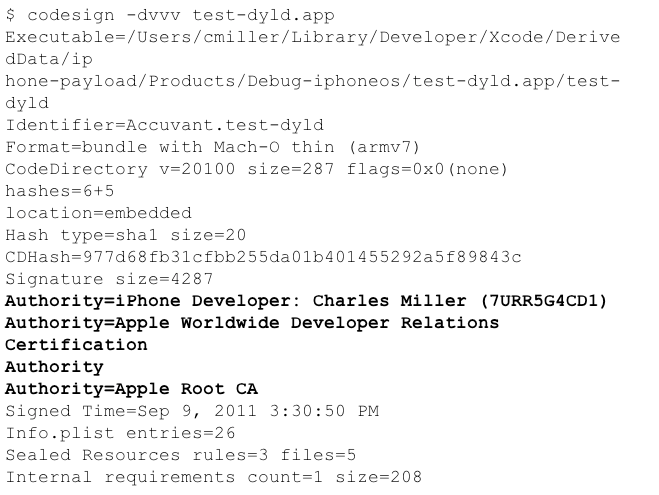
\includegraphics[scale=0.6]{developerZert-codesign-CDHash.png}
        \caption{Developer signed CDHash (Vgl. \cite{Hacking[1]})}
        \label{fig:Developer signed CDHash}
\end{figure}

Es besteht immer die Möglichkeit, dass eine App von Apple bzw. einem anderen Entwickler re-signiert wird.\cite{Sign[1], Sign[2], Sign[3], Sign[4], Sign[5]}. Die Abbildung \ref{fig:Apple signed CDHash} zeigt eine App die von Apple signiert und via iTunes verteilt wurde.

\begin{figure}[!ht]
        \centering
        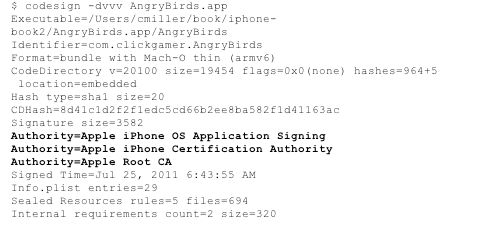
\includegraphics[scale=1.0]{AppleZert_CDHash.png}
        \caption{Apple signed CDHash (Vgl. \cite{Hacking[1]})}
        \label{fig:Apple signed CDHash}
\end{figure}

Die Abbildung \ref{fig:Ad-Hoc CDHash} zeigt eine App ohne Informationen betreffend des Zertifikates, mit welchen die App signiert wurde. Es ist nur der CDHash verfügbar und das Entitlement adhoc ist gesetzt. Dies bedeutet, dass dieser CDHash im \textit{\glqq static trusted cache\grqq{}} enthalten ist. (Vgl. \cite{Sign[1], Sign[2], Sign[3], Sign[4], Sign[5]})

\begin{figure}[!ht]
        \centering
        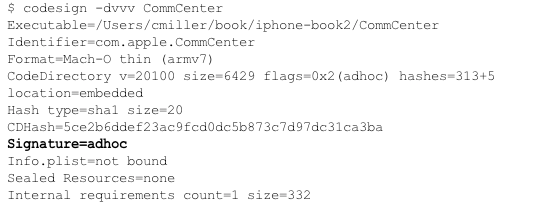
\includegraphics[scale=0.9]{ADhoc_CDHash.png}
        \caption{Ad-Hoc CDHash (Vgl. \cite{Hacking[1]})}
        \label{fig:Ad-Hoc CDHash}
\end{figure}

%------------------------------------------------------------------------------
%------------------------------ Encryption and Data Protection
\section{Datenverschlüsselung und -schutz}
\label{sec:EncryptionandDataProtection}

In den Kapiteln zuvor wurden die Sicherheitsmechanismen beschreiben, die sicherstellen, dass nur ein vertrauenswürdiger Code auf dem Device ausgeführt werden kann. Dieses Kapitel befasst sich mit der Sicherheit von Userdaten auf dem iOS Device. 

Ab der iOS Version 8 wurde die verpflichtende Verschlüsselung von Userdaten eingeführt. Die iOS Produkte verfügen über unterschiedliche Schutzmechanismen, sowohl im Betriebssystem, als auch im iOS Device. Wenn alle anderen Sicherheitsmechanismen umgangen werden, kann trotzdem nicht auf die unverschlüsselten Userdaten zugegriffen werden. Dies ist der Datenverschlüsselung und dem Datenschutz-Mechanismus zuzuschreiben.

\subsubsection{Hardware Security Protection}
\label{sec:HardwareSecProtection}

Jedes iOS Device hat eine eigene \textbf{AES 256 Crypto Engine}. Diese Crypto Engine ist Teil des \textit{\glqq Direct Memory Access(DMA)\grqq{}} Pfades und wurde zwischen dem \textit{\glqq Main System Memory(Hauptspeicher des Systems)\grqq{}} und dem \textit{\glqq Flash Memory\grqq{}} angeordnet. Das ermöglicht es, dem iOS Device die sehr teuren und komplexen kryptographischen Operationen effizient und energiesparend durchzuführen.(Vgl. \cite{iOSSec[5], iOSSec[2],iOSSec[1], Apple[4], Apple[5], Apple[6], Apple[3]})

Während der Herstellung des Applikationsprozessors und der Secure Enclave wird die \textit{\glqq Unique ID\grqq{}} (UID, eindeutige ID des Gerätes) und die \textit{\glqq device Group ID\grqq{}} (GID, Gerätegruppen ID) in die Hardware gebrannt oder kompiliert. Die GID ist für alle Prozessor Geräteklassen gleich, so haben alle Apple A8 die selbe GID. \par 
Die UID und die GID bestehen aus \textbf{AES 256-Bit Keys}. Es ist für keine Software oder Firmware möglich, diesen Key direkt auszulesen. Es können nur die Ver- und Entschlüsselung-Funktionen verwendet werden, die von der AES Engine zur Verfügung gestellt werden. (Vgl. \cite{iOSSec[5], iOSSec[2],iOSSec[1], Apple[4], Apple[5], Apple[6], Apple[3]})

Der \textbf{Secure Enclave} ist ein \textbf{Coprozessor} des \textit{\glqq Apple A7 Prozessors\grqq{}} und der späteren \textit{\glqq A-Serie Prozessoren\grqq}. Jeder Secure Enclave hat ihre eigene UID, die bei der Herstellung des Koprozessors gebrannt wird.

\newpage
\begin{description}
     \item[\parbox{\textwidth} {Die Secure Enclave hat folgende Aufgaben}]~\par
    \begin{enumerate}
        \item Die Zurverfügungstellung der kryptographischen Verfahren für die Schlüsselverwaltung (File Key Siehe Kapitel: \ref{sec:DataProtection}).
       \item Die Verwaltung der Fingerabdruckdaten (Touch-ID Siehe Kapitel: \ref{sec:Passcode}).
       \item Die Daten, die von der Secure Enclave im Dateisystem gespeichert werden, werden mit einem Schlüssel verschlüsselt, der mit der UID und einem \textit{\glqq Anti-Replay-Zähler\grqq{}} verknüpft ist.
       \item Die Verifikation des AES 256 verschlüsselten User Passcode
    \end{enumerate}   
\end{description} 

Alle anderen kryptographischen Keys werden vom \textit{\glqq Random Number Generator(RNG)\grqq{}} erzeugt. Der RNG basiert auf dem \textit{\glqq AES 256 CTR\_DRBG Algorithmus\grqq{}}.(Vgl. \cite{iOSSec[5], iOSSec[2],iOSSec[1], Apple[4], Apple[5], Apple[6], Apple[3]})

Durch die Verschachtelung der UID mit dem AES 256-Bit Key ist es nicht möglich, den Flash Memory in ein anderes iOS Device einzubauen und dann die Userdaten zu dekodieren. Somit können die Userdaten nur auf dem Device mit dem Koprozessor mit der entsprechenden UID entschlüsselt werden. (Vgl. \cite{iOSSec[5], iOSSec[2],iOSSec[1], Apple[4], Apple[5], Apple[6], Apple[3]})

\subsubsection{Datenschutz}
\label{sec:DataProtection}

Zusätzlich zur Hardware Protection stellt Apple eine weitere Sicherheitstechnologie für iOS Geräte zur Verfügung, diese wird \textbf{Data Protection}(Datenschutz) genannt. Ab der iOS Version 7.0 wird Data Protection für alle Third-Party Apps defaultmäßig aktiviert.(Vgl. \cite{iOSSec[5], iOSSec[2],iOSSec[1], Apple[4], Apple[5], Apple[6], Apple[3]})

\paragraph{Datenschutz} wurde speziell für mobile Geräte entwickelt. iOS entschlüsselt immer nur die Daten, die gerade von Apps/Prozessen verwendet/benötigt werden. Dies hat den Vorteil, dass bei einem Event (zB. eingehender Anruf) nicht die gesamte Daten entschlüsselt werden müssen, um diesen Event behandeln zu können. (Vgl. \cite{Apple[4]})

\paragraph{File Datenschutz} basiert auf dem Datenschutz-Mechanismus, dieser wiederum beruht auf einer hierarchischen Schlüsselverteilung. Mit dem Erstellen eines neuen Files auf der Datenpartition wird auch ein neuer \textit{\glqq File Key 256-Bit\grqq{}} (\glqq File Key\grqq) erzeugt. Dieser wird der Hardware AES Engine übergeben und dann zur Verschlüsselung des Files verwendet.  Der \textit{\glqq AES-CBC Mode\grqq{}} wird verwendet, um das File auf den Flash Memory zu schreiben. Der A8 Prozessor verwendt hierfür den \textit{\glqq AES-XTS Mode\grqq{}}.  \par
Der \textbf{Initialisierungsvektor(IV)} wird mit Hilfe des Block Offset der Datei berechnet, und zur Verschlüsselung wird der SHA-1 Hash des \textit{\glqq File Keys\grqq{}} verwendet. (Vgl. \cite{iOSSec[5], iOSSec[2],iOSSec[1], Apple[4], Apple[5], Apple[6], Apple[3]})

Der Content des Files wird mit dem \textbf{File Key} verschlüsselt. Dieser wird mit einem \textbf{Class Key} verpackt (wrapped) und in den Metadaten des Files gespeichert. Die Metadaten werden mit dem \textbf{File System Key} verschlüsselt. Der Class Key ist mit dem \textbf{Hardware Key} geschützt. Manche Klassen werden zusätzlich noch mit \textbf{Passcode Key} gewrapped.(Vgl. \cite{iOSSec[5], iOSSec[2],iOSSec[1], Apple[4], Apple[5], Apple[6], Apple[3]})
\begin{figure}[hp!]
        \centering
        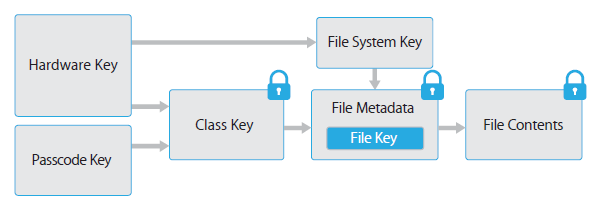
\includegraphics[scale=0.75]{fileDataProtection.PNG}
        \caption{File Data Protection (\cite{Apple[4]} S.11)}
        \label{fig:FileDataProtection}
\end{figure}

\subsubsection{Passcode}
\label{sec:Passcode}

Mit dem Aktiveren dws Passcodes wird der Datenschutz des iOS Devices aktiviert. 
\begin{description}
    \item[\parbox{\textwidth} {Der User hat die Möglichkeit, zwischen drei Einstellungsvarianten des Passcodes zu variieren}]~\par
   \begin{enumerate}
        \item eine vierstellige Zahl,
        \item eine sechsstellige Zahl und
        \item eine beliebige Anzahl alphanumerischer Zeichen.
    \end{enumerate}
\end{description} 

Die Sicherheit des iOS Devices hängt mit der Sicherheit des Passcodes zusammen. Je stärker der Passcode ist umso stärker ist auch der Verschlüsselungskey. 

\subsection{Sandbox}
\label{sec:Sandbox}

\textbf{Die Sandbox} ist ein weiterer Zugriffkontrollmechanismus, um Userdaten zu schützen. Die Sandbox wird auch als \textbf{Last Line of Defense} bezeichnet. Wenn alle anderen Sicherheitsmechanismen schon versagt haben, verhindert die Sandbox ein Übergreifen der Schadsoftware auf das gesamte Device. Die Schadsoftware kann sich nur in den Verzeichnissen der App ausbreiten. Die Malware kann nur auf die Daten in diesem Verzeichnisbaum zugreifen, und es stehen auch nur die Systemressourcen zur Verfügung, die für diese App vom Entwickler festgelegt wurden. \par
Würde eine Schadsoftware Zugriff auf eine App erhalten, die in keiner Sandbox läuft, so hätte die Malware Zugriff auf alle Daten des Devices und könnte alle Systemressourcen uneingeschränkt verwenden.\par
Fabin Vogt beschreibt dies in seiner Abhandlung so: \textit{\glqq Dealing with faults in software is a complicated task, especially when a system may be extended by various modules. These modules may contain unforeseen faults and thus portray a serious threat to the overall system reliability and security. So the main goal for software fault isolation is to limit the impact of module faults to a small part of the system. The untrusted module is therefore loaded in its own fault domain [9], which is logically separated from the rest of the system.\grqq{}} \cite{Sandbox[4]}

\begin{description}
    \item[\parbox{\textwidth} {Unter anderem könnte die Malware folgende Systemressourcen unbemerkt vom User verwenden}]~\par
    \begin{itemize}
        \item die eingebaute Kamera
        \item das eingebaute Mikrophon
        \item die Network Sockets
        \item und auch die meisten Bereiche des File Systems.
    \end{itemize}
\end{description} 
(Vgl. \cite{Apple[6], Sandbox[1], Sandbox[2],Sandbox[3], Sandbox[4], Sandbox[5], Sandbox[6]})

\begin{figure}[hp!]
        \centering
                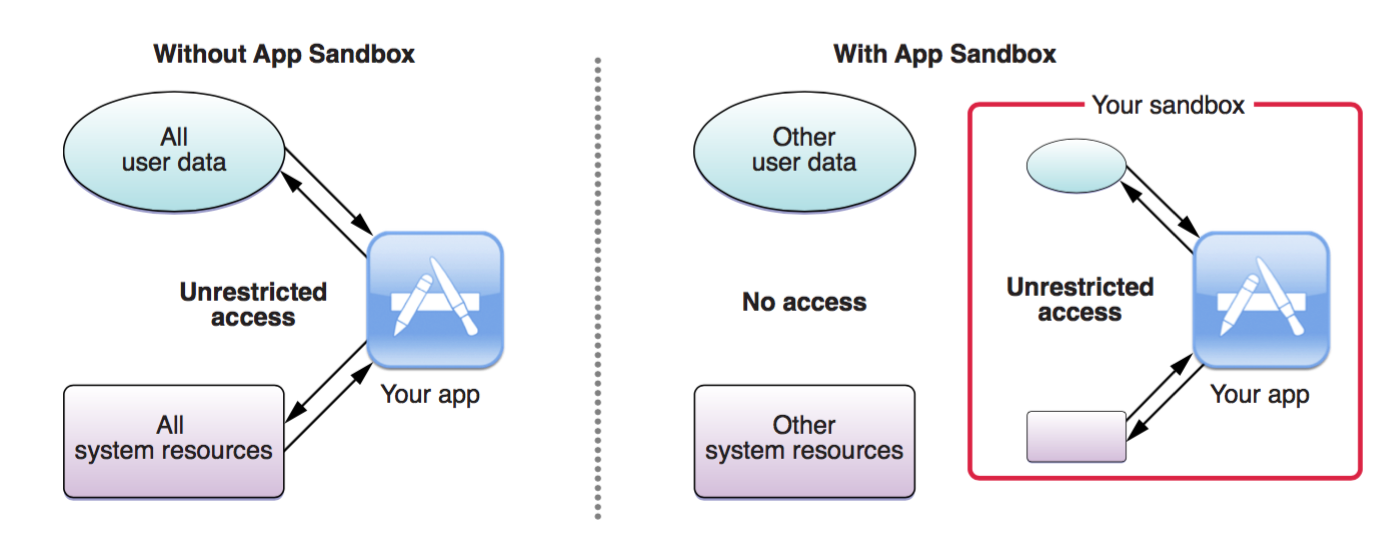
\includegraphics[scale=0.5]{iOSsandbox}
        \caption{iOS Sandbox (Vgl. \cite{Sandbox[3]}, S.6)}
        \label{fig:iOSsandbox}
\end{figure}

\begin{description}
    \item[\parbox{\textwidth} {Wenn eine Sandbox für eine App vom iOS angelegt wird, stehen der App folgende Container Verzeichnisse zur Verfügung}]~\par
    \begin{enumerate}
        \item \textbf{ App Container Directory:} \\
        Beim ersten Starten der App wird vom Betriebssystem ein Verzeichnis erstellt, dieses kann nur von dieser App verwendet werden. Dies wird als Container bezeichnet. Jeder User des Systems erhält seinen eigenen Container für diese App.
        \item \textbf{ App Group Container Directory:} \\
        Mit Hilfe von Entitlements kann konfiguriert werden, welche Apps Zugriff auf den Group Container haben. Dieser Container dient zum Datenaustausch zwischen unterschiedlichen Apps.
        \item \textbf{Diverse System Verzeichnisse}
    \end{enumerate}
\end{description} 


%\subsection{Schutzklassen}
%\label{sec:Schutzklassen}

%\subsection{Remote Wipe}
%\label{sec:RemoteWipe}

%\subsection{Collecting Signing}
%\label{sec:CollectingSigning}

%\subsection{Verifying Signing}
%\label{sec:VerifyingSigning}

%\subsection{Dynamic Code Signing}
%\label{sec:DynamicCodeSigning}

%\subsection{Runtime Process Security}
%\label{sec:RuntimeProcessSecurity}



%------------------------------------------------------------------------------
%------------------------------  Stack Guard ----------------------------------
%\section{Stack Guard}
%\label{sec:StackGuard}
%\subsection{Stack}
%\label{sec:Stack}
%\subsection{Heap}
%\label{sec:Heap}
%
%------------------------------------------------------------------------------
%------------------------------  NetworkSecurity
%\section{Network Security}
%\label{sec:NetworkSecurity}
%
%\subsection{Secure Socket Layer}
%\label{sec:SSL}
%
%\subsection{Transport Layer Security}
%\label{sec:TLS}
          % iOS Sicherheit Konzept
%----------------------------------------------------------------
%
%  File    :  chapter6.tex
%
%  Authors : Michael Fuska, FH Campus Wien, Austria
%  Created : 13 Feb 2016
%
%  Changed :  
% 
%----------------------------------------------------------------


\chapter{Analyse und Ergebnisse}
\label{ch:Ergebnisse}

%------------------------------------------------------------------------------
%------------------------------ Analysen zur Frage 1

\section{Welche Faktoren sind für die Sicherheit und die Vertrauenswürdigkeit eines iOS Device ausschlaggebend?}
\label{sec:Frage1}

\begin{table}[htp!]
    \begin{center}
        \begin{tabular}{|p{30mm}|p{27mm}|p{12mm}|p{10mm}|p{18mm}|p{2cm}|p{15mm}|} \hline
            \textbf{iOS Device} & \textbf{Verkaufsstart} & \textbf{initial iOS} & \textbf{last iOS} & \textbf{Secure Enclave} & \textbf{Prozessor}  & \textbf{\#Tage JB} \\ \hline
            \textbf{iPhone} & 29.06.2007  & 1.0 & 3.1.3 & nA & Samsung SSL8900 & 11\\ \hline
            \textbf{iPhone 3G} & 11.07.2008 & 2.0 & 4.2.1 & nA & Samsung SSL8900 & 9\\ \hline
            \textbf{iPhone 3GS} & 19.06.2009 & 3.0 & 6.1.6 & nA & Samsung SSL8920 & 14\\ \hline
            \textbf{iPhone 4} & 01.08.2010 & 4.0 & 7.1.2 & nA & Apple A4 & 38 \\ \hline
            \textbf{iPhone 4s} & 20.01.2012 & 5.0 & 9.3.2 & nA & Apple A5 & 98 \\ \hline 
            \textbf{iPhone 5} & 21.09.2012 & 6.0 &  9.3.2 & nA & Apple A6 & 136 \\ \hline
            \textbf{iPhone 5c} & 22.12.2013 & 7.0 & 9.3.2 & nA & Apple A6 & 93 \\ \hline
            \textbf{iPhone 5s} & 22.12.2013 & 7.0 & 9.3.2 & A & Apple A7 & 93 \\ \hline
            \textbf{iPhone 6} & 19.09.2014 & 8.0 & 9.3.2 & A & Apple A8 & 33\\ \hline
            \textbf{iPhone 6 Plus} & 19.09.2014 & 8.0 & 9.3.2 &  A & Apple A8 & 33\\ \hline
            \textbf{iPhone 6s} & 25.09.2016 & 9.0 &  9.3.2 & A & Apple A9 & 19\\ \hline
            \textbf{iPhone 6s Plus} & 25.09.2016 & 9.0 & 9.3.2 &  A & Apple A9 & 19\\ \hline
            \textbf{iPhone SE} & 31.03.2016 & 9.0 &  9.3.2 & A & Apple A9 & nA\\ \hline  
        \end{tabular} 
        \caption{Auflistung iOS Device/ Verkaufsstart/ initial iOS/ last supported iOS / Prozessor/ \#Tage bis zum JB}
        \label{tab:iOSHW}
    \end{center}
\end{table}

In der Tabelle \ref{tab:iOSHW} werden alle iOS Devices aufgelistet und  in Abhängigkeit vom Verkaufszeitpunkt des Device, der initial installierten iOS Version und des Prozessor-Typs des iDevice gebracht. Zusätzlich wird in der Tabelle angeführt, ob diesem Device einen Koprozessor mit Secure Enclave zur Verfügung steht und wie lange die JB Community benötigte, um ein JB für dieses Device zu veröffentlichen. Diese Tabelle beinhaltet alle Daten die als Grundlage für alle weiteren Analysen in diesem Kapitel dienen.\par


%------------------------------------------------------------------------------
%------------------------------ 
\subsection{iOS Device (G1.1)}
\label{sec:Frage1iOSDevice} 

Die Tabelle \ref{tab:iOSHW} alleine gibt noch keinen Aufschluss über den Zusammenhang zwischen der Sicherheit des Systems und der verwendeten iOS Hardware. Da die Tabelle \ref{tab:iOSHW} keine Aussagen darüber zulässt, ob der Zeitraum bis zum Veröffentlichen des JB nur von der HW abhängt oder von der iOS Version die am Device installiert wurde. Aus diesem Grund müssen die Daten der beiden Tabellen (Tabelle: \ref{tab:iOSHW}, Tabelle: \ref{tab:iOSVersion}) korreliert werden. \par 
\begin{table}[htp!]
    \begin{center}
        \begin{tabular}{|l|l|l|} \hline
         \textbf{iOS Version} & \textbf{Veröffentilicht} & \textbf{\#Tage JB}\\ \hline    
        1.0 & 29.06.2007 & 11\\ \hline 
        2.0 & 11.07.2008	& 9\\ \hline 
        3.0 & 17.06.2009	& 2\\ \hline 
        4.0 & 21.06.2010 & 2\\ \hline 
        5.0 & 12.10.2011	& 1\\ \hline 
        6.0 & 19.09.2012	& 0\\ \hline 
        7.0 & 18.09.2013	& 95\\ \hline 
        7.1-7.1.2 & 29.05.2014 & 25\\ \hline 
        8.0 & 17.09.2014	& 35\\ \hline 
        8.1.1-8.4 & 17.11.2014	& 12\\ \hline 
        9.0 & 16.09.2015	& 28\\ \hline
       %  9.0.1 & 23.09.2015 & nA \\ \hline
       %  9.0.2 & 30.09.2015 & nA \\ \hline 
        9.1 & 21.10.2015	& 142\\ \hline 
       %  9.2 & 08.12,2015 & nA\\ \hline
       % 9.2.1 & 18.02.2016 & nA \\ \hline
       %  9.3 & 21.03,016 & nA\\ \hline 
       % 9.3.1 & 31.03.2016 & nA\\ \hline
       % 9.3.2 & 17.05.2016 & nA \\ \hline
        \end{tabular} 
        \caption{Auflistung iOS Version/ Veröffentlichungsdatum/ \# Tage bis zum JB}
        \label{tab:iOSVersion}
    \end{center}
\end{table}

Die Tabelle \ref{tab:iOSVersion} listet die iOS Version, das Veröffentlichungsdatum dieser iOS Version und die Anzahl an Tagen die benötigt wurden, um einen JB für diese iOS Version zu veröffentlichen auf.  \par 
\begin{figure}[htbp]
        \centering
                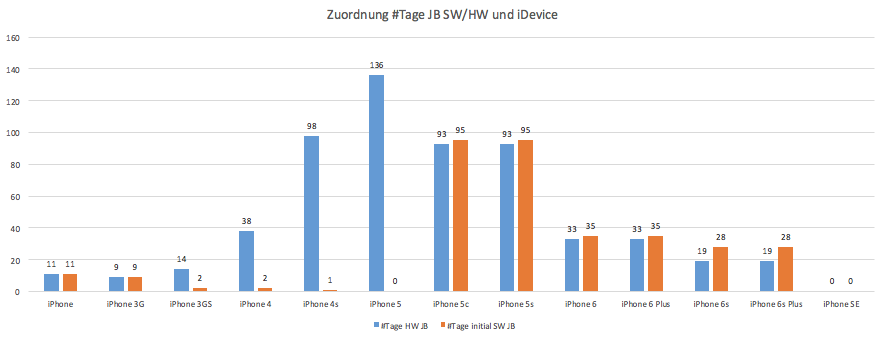
\includegraphics[scale=0.55]{Bilder/iDeviceJB-SW-HW.png}
         \caption{Vergleich der Anzahl der Tage eines JB für die Prozessoren und für der initialen iOS Version}
        \label{fig:VergleichJBProzessorSW}      
\end{figure}
Die Abbildung \ref{fig:VergleichJBProzessorSW} stellt die Verbindung zwischen dem Prozessoren des iDevices, der installierten iOS Version und der benötigten Tage für die Veröffentlichung eines JB her. Es kann gezeigt werden, dass alle Apple Prozessorarchitekturen einschliesslich des Apple A6 ein Sicherheitsgewinn für die iOS Produkte bedeutet haben. Dieser Schluss ist darauf begründet, dass die JBs für die selbe iOS Version auf älteren Apple Prozessorarchitekturen innerhalb von wenigen Tagen verfügbar war. \par 
Eine Veränderung ist in den Daten ist ab dem Apple A7 Prozessors sichtbar. Da zwischen dem veröffentlichen des JBs für die iOS Hardware und die iOS Version, nur mehr eine marginale Unterschied vorliegt.
\paragraph{Ergebnisse:} Dies lässt den Schluss zu, dass die Sicherheit und die Vertrauenswürdigkeit der iOS Produkte zum heutigen Zeitpunkt nur mehr von Apples mobilen Betriebssystem abhängt und nicht von der verwendeten iOS Hardware. 
% TODO
%64 BIT Architektur
%
%------------------------------------------------------------------------------
%------------------------------ 
\subsection{Secure Enclave  (G1.1)}
\label{sec:Frage1SecureEnclave}
 
 Unter iOS gibt es die Möglichkeit verschiedene Passcode Konfigurationen vorzunehmen. Abhängig davon welche Prozessorgeneration verwendet wird, werden die Konfiguration und Daten des Passocdes in einer \textbf{Secure Enclave} oder im Flash Memory gespeichert. Neben der Anzahl der Stellen, kann auch konfiguriert werden, ob nur Zahlen oder auch alphanumerische Werte für einen Passcode verwendet werden.\par 
 Ein weiterer iOS Konfigurationsparameter ermöglicht es, das Device so zu konfigurieren, dass nach zehn falschen Passcode Eingaben alle Daten des Gerätes gelöscht werden. Die Anzahl der Fehlversuche wird bei iOS Devices ohne Secure Enclave in den Flash Memory geschrieben. Bei iOS Devices mit Secure Enclave werden diese Daten in der \textit{\glqq ARM Trust Zone\grqq{}} gespeichert und können somit nicht ohne weiters ausgelesen und überschrieben werden. 
 
% Die Secure Enclave des Koprozessor (siehe Tabelle: \ref{tab:iOSHW}) bringen einen massiven Sicherheitsgewinn für die iOS Produkte mit sich, da die  
 
 Im Fall \textit{\glqq FBI gegen Apple\grqq{}} wurde der Tatsache, dass das iOS Device keine Secure Enclave enthält, besonderer Bedeutung beigemessen. Das FBI beauftragte ein Unternehmen um das iPhone 5c des Attentäters zu entsperren. Die Abbildung: \ref{fig:iOSSecurityArchitekturiOS7} zeigt die iOS Sicherheitsarchitektur des iPhone 5c. Die Systemarchitektur dieses iOS Device beinhaltet keine Secure Enclave. \par 
\begin{description}
    \item[\parbox{\textwidth} { Der Sicherheitsforscher Zdziarski beschreibt in seinen Abhandlungen die plausiblen Varianten des FBI Hacks wie folgt}]~\par
    \begin{enumerate}
        \item \textit{\glqq .... based on all of this, is that an external forensics company, with hardware capabilities, is likely copying the NAND storage off the chip and frequently re-copying all or part of the chip’s contents back to the device in order to brute force the pin – and may or may not also be using older gear from iOS 8 techniques to do it. The two weeks the FBI has asked for are not to develop this technique (it’s most likely already been developed, if FBI is willing to vacate a hearing over it), but rather to demonstrate, and possibly sell, the technique to FBI by means of a field test on some demo units.\grqq{}} \cite{Hacking[4]}
        \item \textit{\glqq If the FBI did in fact use a software exploit, the question then becomes one of how viable it is on other platforms.\grqq{}} \cite{Hacking[4]}
    \end{enumerate}
\end{description} 

\paragraph{Ergebnisse:} Die Secure Enclave biete einen Sicherheitsgewinn für die iOS Produkte, aber der Fall \textit{\glqq FBI via Apple\grqq{}} lässt einige Fragen offen. Da das FBI, Apple die Sicherheitslücke nicht offenlegte gibt es nur Mutmaßungen, über den Hack der verwendet wurde, um das iPhone des Attentäters zu entsperren. \par 

Zdziarski beschreibt die möglichen Folgen dieses Hacks wie folgt: \textit{\glqq The moral of the story is that the exploit the FBI may have is dangerous in and of itself, regardless of whether it serves their specific purposes of brute forcing a device’s pin. Such an exploit has numerous uses within the intelligence community and poses a threat to not only the hundreds of millions of older devices out there, but if it can be ported to a 64-bit platform, every single one of us – either directly as a threat from the government, a nation state the exploit developer also sold it to, or another hacker who finds the same hole because FBI didn’t report the vulnerability to Apple. FBI has left us all potentially exposed by choosing to keep their technique secret.\grqq{}} \cite{Hacking[4]} \par 

Vor allem gibt es Vermutungen, dass der Hack des FBIs eine Möglichkeit bietet die Secure Enclave zu umgehen.


\newpage
%------------------------------------------------------------------------------
%------------------------------ 
\subsection{iOS Version  (G1.2)}
\label{sec:Frage1iOSVersion} 

\begin{figure}[hp!]
        \centering
                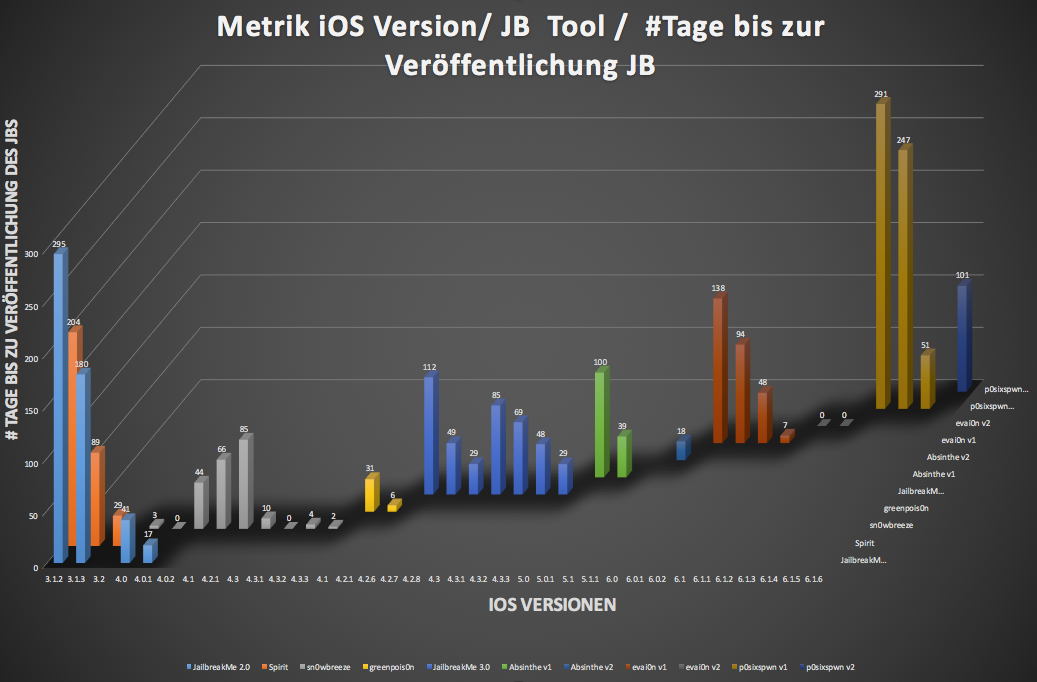
\includegraphics[scale=0.38]{Bilder/Frage1_1.png}
        \caption{iOS Version / JB Tools /\# Tage bis zum JB}
        \label{fig:AnalyseiOSJB1}        
\end{figure}

\begin{figure}[hp!]
        \centering
                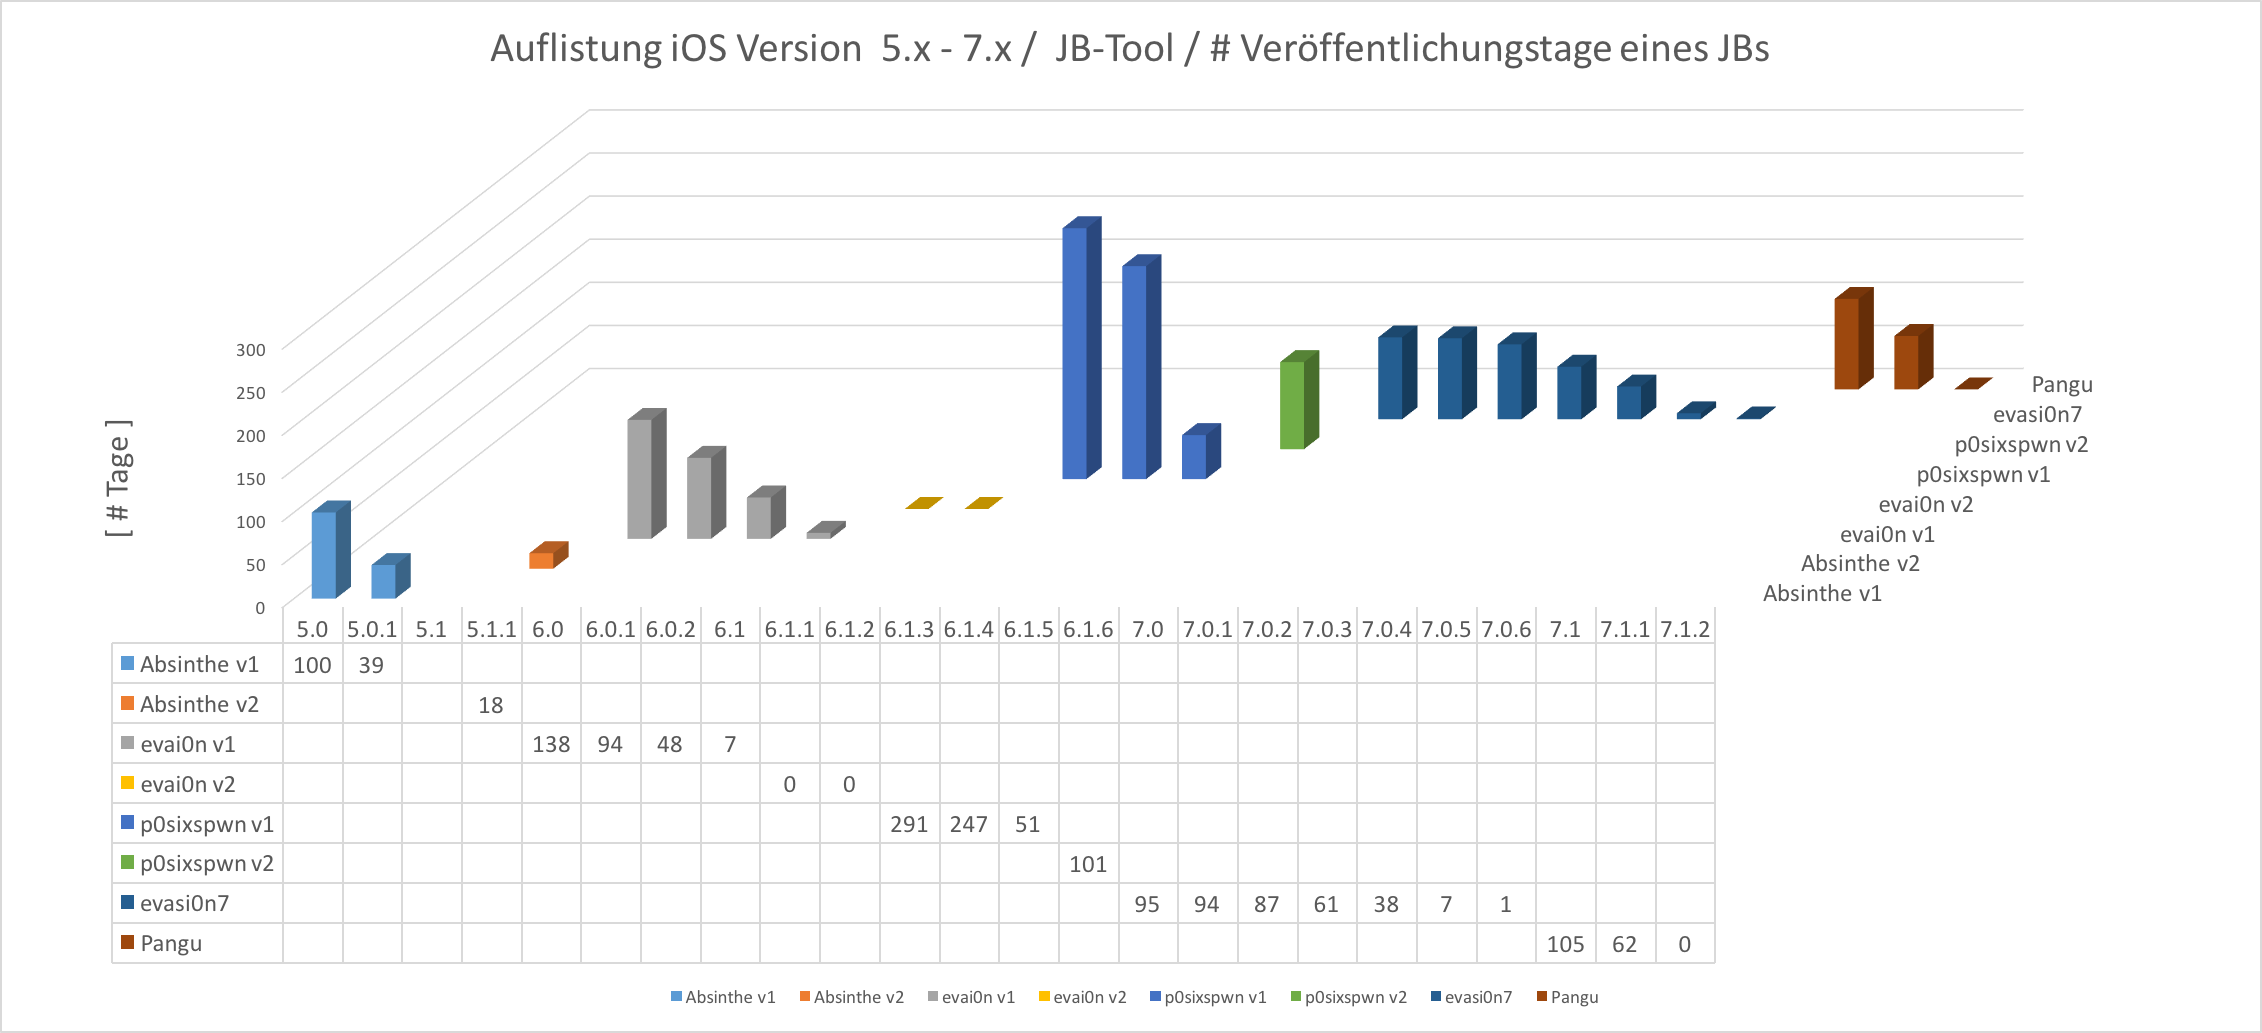
\includegraphics[scale=0.35]{Bilder/Frage1_2.png}
        \caption{iOS Version / JB Tools /\# Tage bis zum JB}
        \label{fig:AnalyseiOSJB2}
\end{figure}

Die Abbildungen \ref{fig:AnalyseiOSJB1} und \ref{fig:AnalyseiOSJB2} zeigen die bekanntesten und stabilsten untethered JBs, in Abhängigkeit mit der iOS Version und der Anzahl an Tagen die benötigt wurden, um für diese iOS Version ein Jailbreak bereitzustellen. \par 
\textbf{Die Graphiken zeigen,} dass ein JB immer nur für eine Serie von iOS Version funktioniert. In den meisten Fällen funktioniert der JB für die \textit{\glqq aktuelle\grqq{}} iOS Version und einigen iOS Versionen davor. Nach wenigen Wochen stellt Apple ein iOS Sicherheitsupdate zur Verfügung, welches das JB verhindert. Dieses Verhalt zieht sich durch alle betrachtet Metriken.  
%
%dass nach einem gelungen JB die Sicherheitsupdates von Apple einen kurzzeitigen Sicherheitsmehrwert mit sich bringen, aber innerhalb einiger Tage wurde ein neuer JB, des selben JB-Team veröffentlicht. Dies lässt darauf schliessen, dass die Sicherheitslücken nur teilweise geschlossen worden sind. Dieser Verhalten gilt  für alle iOS Versionen bis einschliesslich der iOS Version 9.x.\par  
%Ab der iOS Version 8.x ändert sich dieses Verhalten, da die JB Community jetzt länger für die JBs der nachfolgenden iOS minor Releases benötigt. \par 
%Markant ändern sich die Muster ab der iOS Version 9.x. Das JB für die Minor iOS Version 9.1 benötigte fast sechsmal länger, als das JB für die Major iOS Version 9.0 benötigte.\par



\begin{figure}[hp!]
        \centering
                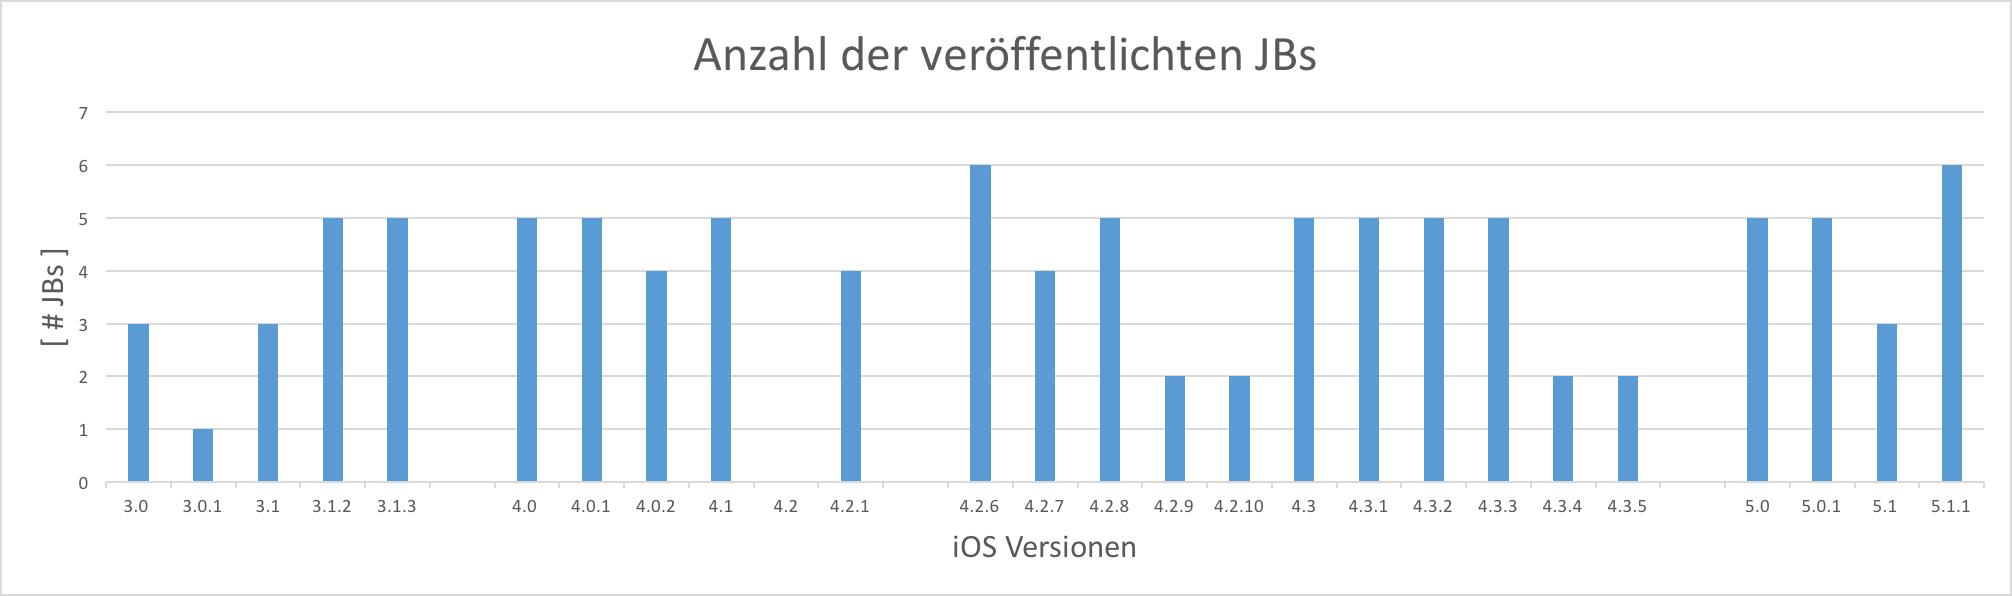
\includegraphics[scale=0.5]{Bilder/iOSJB1.png}
        \caption{Anzahl der veröffentlichten JBs pro iOS Version 3.x - 5.1.1}
        \label{fig:AnalyseAnzahliOSJB1}
\end{figure}

\textbf{Die Abbildungen \ref{fig:AnalyseAnzahliOSJB1} und \ref{fig:AnalyseAnzahliOSJB2} zeigen,} dass die Anzahl der veröffentlichten JB-Tools, ab der iOS Version 7.0 massiv rückgängig sind. Es wurden nur mehr ein oder zwei JB-Tools pro iOS Version der Öffentlichkeit zur Verfügung gestellt. 

\begin{figure}[hp!]
        \centering
                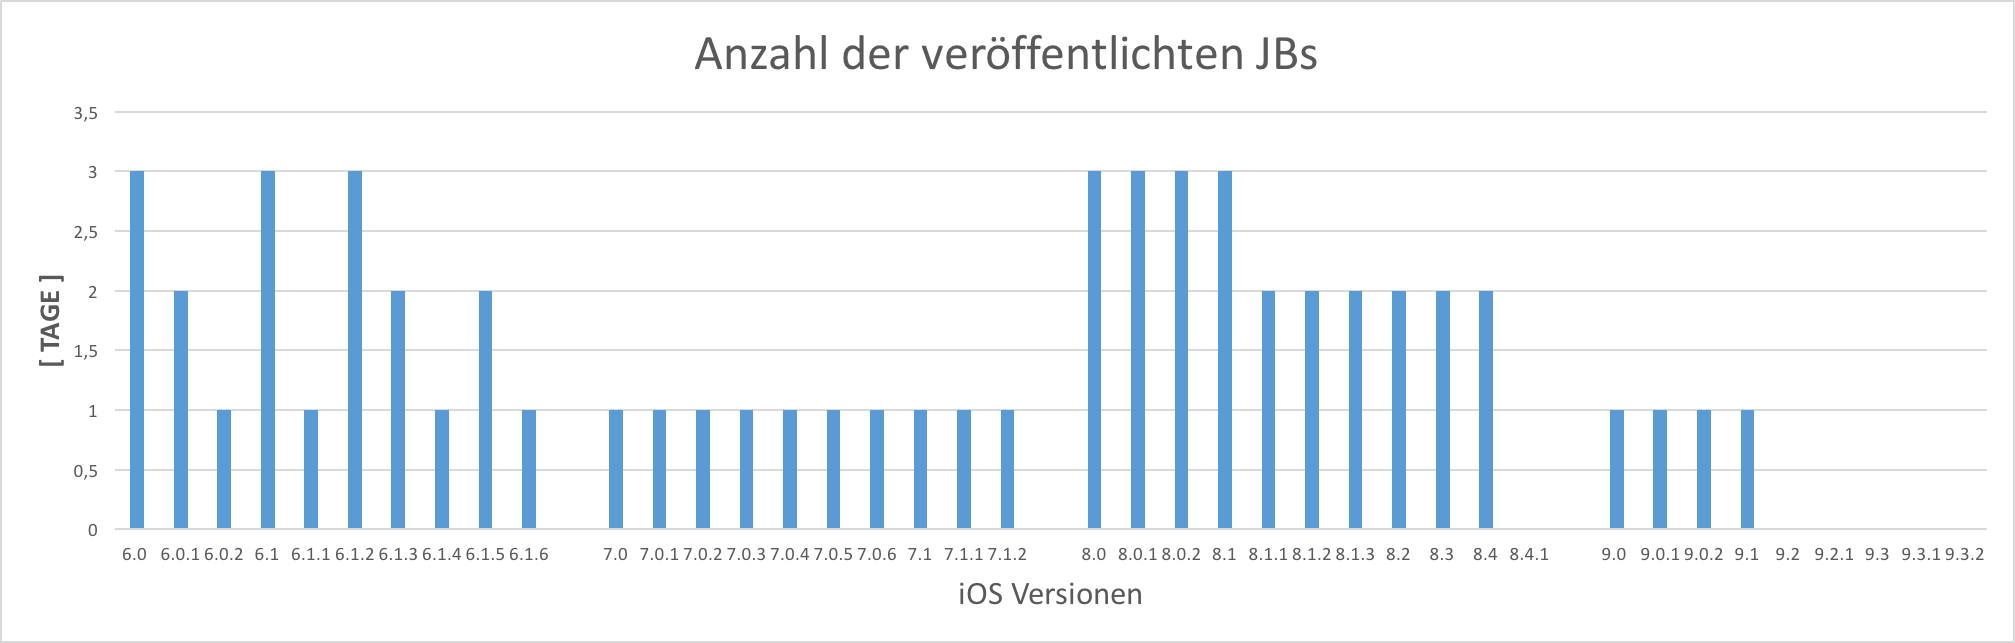
\includegraphics[scale=0.5]{Bilder/iOSJB2.png}
        \caption{Anzahl der veröffentlichten JBs pro iOS Version 6.x - 9.x.x}
        \label{fig:AnalyseAnzahliOSJB2}
\end{figure}


\paragraph{Ergebnisse:} Die aufbereitet Daten lassen den Schluss zu, dass die Sicherheit und die Vertrauenswürdigkeit der iOS Produkte mit steigender iOS Version zunimmt. Dieser Schluss ist darauf begründet, dass die Anzahl der Tage die benötigt wurden, um einen JB zur Verfügung zu stellen, eine steigende Tendenz aufweisen. Der letzte untethered JB wurde Anfang Dezember 2015 veröffentlicht, seit diesem Zeitpunkt wurden sechs iOS Versionen veröffentlicht und es sind 243 Tage (per 18.07.2016) vergangen.\par 
Ein weiterer Anhaltspunkt für die Steigerung der Sicherheit ist, dass die Anzahl der Menschen die noch einen funktionsfähigen Jailbreak entwickeln können sinkt. 
\par 
Es muss darauf hingewissen werden, dass Apple seine Strategie im Bezug auf die JB Community geändert hat. In der Vergangenheit hat Apple versucht, gegen JBs gerichtlich vorzugehen, aber nur mit begrenzten Erfolg (\textit{\glqq Klage gegen George Hotz alias Geohot\grqq{}}). Apple hat vor einigen Jahren damit begonnen namhafte iOS Hacker anzustellen, unteranderem Comex  der Entwickler von \textit{\glqq JailbreakMe\grqq}. Dies bringt zwei Vorteile für Apple mit sich. Erstens, die Hacker kennen das mobile Betriebssystem und die Schwächen dieses, besser als viel interne Apple Entwickler.  Zweitens, die JB Community verliert ein aktives Mitglied. Als sehr viel schwerwiegender für die JB-Community einzustufen ist, dass durch den ehemaligen Hacker auch einige Zero-Day Bugs Apple gemeldet werden.\par
Seit dem Jahr 2015 ist der kommerzielle Aspekt in diesem Zusammenhang nicht ausser acht zu lassen. Angefangen mit dem Preisgeld welches auf ein JB der iOS Version 9.x ausgesetzt wurde, bis hin zu Premieren für Zero-Day Bugs. Dies hat meiner Meinung nach einen grossen Einfluss auf die Dauer der Veröffentlichung der JBs. Die markanten Ausreißer in den Metriken, ab der iOS Version 9.1 beruhen meiner Meinung nach auf dem kommerziellen Faktor. 

\newpage
%------------------------------------------------------------------------------
%------------------------------ 
\section{Welche Auswirkung haben die von Apple eingeführten Sicherheitsupdates auf die Sicherheit des Systems?}
\label{sec:Frage2}
%------------------------------------------------------------------------------
%------------------------------ 
%\subsection{iOS Sicherheitsmechanismen}
%\label{sec:Frage2SecMechanismen}
% 
%\begin{table}[htp!]
%    \begin{center}
%        \begin{tabular}{|l|l|l|l|} \hline
%            \textbf{Sicherheitsmechanismus} & \textbf{iOS 2.0} & \textbf{iOS 4.3} & \textbf{iOS 8.0} \\ \hline
%             Anzahl behobener Fehler & nA & 12 & 48\\ \hline
%             MAC & 8 & - & - \\ \hline
%             JIT & 8 & 85 & - \\ \hline
%             ASLR & - & 85 & - \\ \hline
%             verpflichtende Datenverschlüsselung & - & - & 35 \\ \hline
%             verpflichtende Datenverschlüsselung & - & - & 73\\ \hline
%        \end{tabular} 
%        \caption{Auflistung Sicherheitsmechanismus}
%        \label{tab:SecMechanismBugs}
%    \end{center}
%\end{table}

%------------------------------------------------------------------------------
%------------------------------ 
\subsection{iOS Sicherheitsupdates  (G1.2)}
\label{sec:Frage2SecUpdate}

In diesem Kapitel wird auf die Wechselbeziehung zwischen der Sicherheit des iOS Device und den JBs, in Abhängigkeit der Hypothese H1 eingegangen. Im Detail wird die Historie einzelner JB-Tool betrachtet. 

\begin{table}[hp!]
    \begin{center}
        \begin{tabular}{| p{20mm} | p{12mm} | p{17mm} | p{12mm} | p{32mm} | p{22mm} | p{15mm} |} \hline
             \textbf{Datum iOS} & \textbf{iOS} & \textbf{\# Bugs} & \textbf{\# JB Bugs} & \textbf{JB Tool} & \textbf{JB Datum} & \textbf{\# Tage bis JB} \\ \hline 
            10.02.2011 & 4.2.6 &  - & -  & JailbreakMe 3.0 & 02.06.2011 & 112 \\ \hline
             09.03.2011 & 4.3 & 12 & 0 & JailbreakMe 3.0 &	02.06.2011 & 85 \\ \hline
             25.03.2011 & 4.3.1 &  - & - & JailbreakMe 3.0 & 02.06.2011 & 69 \\ \hline
            14.04.2011 & 4.2.7 &  4 & 0 & JailbreakMe 3.0 & 02.06.2011 & 49 \\ \hline
             15.04.2011 & 4.3.2 & 5 & 0 & JailbreakMe 3.0 & 02.06.2011 & 48 \\ \hline
             04.05.2011 & 4.2.8 &  - & - & JailbreakMe 3.0 & 02.06.2011 & 29 \\ \hline
            \textbf{04.05.2011} & \textbf{4.3.3} &  - & -  & \textbf{JailbreakMe 3.0} & \textbf{02.06.2011} & \textbf{29} \\ \hline
            15.07.2011 & 4.3.4 &  1 & 2	 & - & - & - \\ \hline
        \end{tabular} 
        \caption{Analyse JB-Tool JailbreakMe 3.0 \protect\footnotemark}         
        \label{tab:AnalyseJailbreakMe3.0}
    \end{center}
\end{table}
%iOS2011-2012
\footnotetext{\url{https://support.apple.com/de-de/HT204611}}
%\footnote{\label{foot:iOS2011-2012}{\url{https://support.apple.com/de-de/HT204611}}}

\paragraph{JailbreakMe 3.0} ist ein \textit{\glqq webbasierter Userland Exploit\grqq{}} und wurde am 02.06.2011 veröffentlicht. Dieser untethered Jailbreak wurde für die iOS Version 4.3.3 bereitgestellt. Es konnten aber mit diesem Exploit auch die iOS Version 4.2.6-4.3.3 (Siehe Tabelle: \ref{tab:AnalyseJailbreakMe3.0})  \textit{\glqq gejailbreaked\grqq{}} werden. 
Dieser Exploit nutzte einen Fehler im CoreGraphik Framework aus. Dieser ermöglicht es, im Zusammenhang mit dem Lesen eines PDFs, einen beliebigen Code auszuführen. Der IOMobileFrameBuffer hatte einen weiteren Softwarefehler, welcher es den JailbreakMe 3.0 Exploit ermöglichte, Systemprivilegien zu erhalten. Beide Bugs wurde in der iOS Version 4.3.4 \footnote{\label{foot:iOS4.3.4}{\url{https://support.apple.com/de-de/HT202272}}} geschlossen. Ab der iOS Version 4.3.4 ist dieser JB nicht mehr funktionsfähig.
 
\paragraph{Ergebnisse:} Interessant an den Daten der Tabelle \ref{tab:AnalyseJailbreakMe3.0} ist, dass in einem Zeitraum von 112 Tagen sechs iOS Sicherheitsupdates von Apple zur Verfügung gestellt wurden. In dieses sechs Updates wurden insgesamt 21 Bugs behoben. Das Schliessen dieser Sicherheitslücken hatte keine Auswirkung auf den später veröffentlichten JB. Dieses Verhalten zeigen sich in allen Analysen der JB-Tools. \par  
Am 15.07.2011 wurde das iOS Sicherheitsupdate 4.3.4 zum Download zur Verfügung gestellt. In diesem Update wurden insgesamt drei Sicherheitslücken von Apple geschlossen. JailbreakMe 3.0 verwendetet zwei von diesen Bugs und somit war der JB für alle weiteren iOS Version unterbunden. Dies zeigt, das Apple dieses JB-Tools \textit{\glqq reverse engineered\grqq{}} hat und gezielt Sicherheitsupdates zum Unterbinden dieser zur Verfügung stellt. Apple benötigte \textbf{43 Tage} um das Update bereitzustellen. Dadurch wird gezeigt, das die JBs einen direkten Einfluss auf die Sicherheit und Vertrauenswürdigkeit des iOS Systems haben, da Apple anhand der in der Analyse gefunden Bugs, Sicherheitsupdates zur Verfügung stellt. \par 

\begin{table}[hp!]
    \begin{center}
        \begin{tabular}{| p{15mm} | p{20mm} | p{17mm} | p{12mm} | p{20mm} | p{22mm} | p{15mm} |} \hline
            \textbf{iOS} & \textbf{Datum iOS} & \textbf{\# Bugs} & \textbf{\# JB Bugs} & \textbf{JB Tool} & \textbf{JB Datum} & \textbf{\# Tage bis JB} \\ \hline 
7.1 & 10.03.2014 & 20 & 4 & Pangu & 23.6.2014 & 105 \\ \hline
\textbf{7.1.1} & \textbf{22.04.2014} & \textbf{4} & \textbf{0} & \textbf{Pangu} & \textbf{23.6.2014} & \textbf{62} \\ \hline
7.1.2 & 30.06.2014 & 18 & 0 & Pangu & 23.6.2014 & -7 \\ \hline
 & & & & & & \\ \hline
8.0 & 17.09.2014 & 44 & 4 & Pangu8 & 22.10.2014 & 35 \\ \hline
8.0.1 & 24.09.2014 & - & - & Pangu8 & 22.10.2014 & 28 \\ \hline
8.0.2 & 25.09.2014 & - & - & Pangu8 & 22.10.2014 & 27 \\ \hline
\textbf{8.1} & \textbf{20.10.2014} & \textbf{5} & \textbf{0} & \textbf{Pangu8} & \textbf{22.10.2014} & \textbf{2} \\ \hline
8.1.1 & 17.11.2014 & 5 & 3 & - & - & - \\ \hline
 & & & & & & \\ \hline
9.0& 16.09.2015 & 71 & 1 & Pangu9 & 14.10.2015 & 28  \\ \hline
\textbf{9.0.1} & \textbf{23.09.2015} & \textbf{-} & \textbf{-} & \textbf{Pangu9} & \textbf{14.10.2015} & \textbf{21}\\ \hline
9.0.2 & 30.09.2015 & 1 & 0 & Pangu9 & 14.10.2015 & -14 \\ \hline
9.1(32 Bit) & 21.10.2015 & 25 & 2 & Pangu9 & 14.10.2015 & -  \\ \hline
		 & & & & & & \\ \hline				
\textbf{9.1(64 Bit)} & \textbf{21.10.2015} & \textbf{25} & \textbf{2} & \textbf{Pangu9} & \textbf{11.3.2016} & \textbf{142}  \\ \hline
9.2 & 08.12.2015	 & 27 & 3 & - & - & - \\ \hline		
     \end{tabular} 
        \caption{Analyse JB-Tool Pangu \protect\footnotemark}
        \label{tab:AnalysePangu}
    \end{center}
\end{table}
%{\label{foot:iOS2015-2016}
%\footnote{\url{https://support.apple.com/de-de/HT201222}}
\footnotetext{\url{https://support.apple.com/de-de/HT201222}}

\paragraph{Das JB-Team Pangu} veröffentlicht in den letzten zwei Jahren JBs für drei Major iOS Versionen. Bevor das Team Pangu ihren ersten JB veröffentlichte, nahmen die Member des Teams an einem iOS Exploitation Trainings von von Stefan Essers teil \footnote{\url{https://www.sektioneins.de/en/trainings/iosexploitation.html}}. Zu Kontroversen führte dieser JB, da dieser auf den im Training vorgeführten Kernel Exploits beruhte.\par
Bis zum heutigen Datum (18.07.2016) wurden vom Pangu Team vier unterschiedliche JB Version veröffentlicht. Mit diesen vier JBs können zwölf iOS Versionen \textit{\glqq gejailbreaked\grqq{}} werden (siehe Tabelle: \ref{tab:AnalysePangu}).

Die Tabelle \ref{tab:AnalysePangu} zeigt, das selbe Muster, wie in den zuvor analysierten JB-Tool JailbreakMe 3.0. Mit einer Ausnahme, das nächste iOS Sicherheitsupdate 9.0.2 verhinderte nicht den JB der vierzehn Tage zuvor veröffentlicht wurde. \par 
Pangu Team veröffentlichte als erstes JB-Team einen JB für die neue 64 Bit Architektur veröffentlicht. 

\paragraph{Ergebnisse:}  Die iOS Version 7.1.2 ist das letzte Sicherheitsupdate für das iPhone 4. Für dieses Device, ist somit das letzte verfügbare Update, als nicht sicher einzustufen. \par 
Interessant ist auch, dass das iOS Sicherheitsupdate 8.1.1 drei Softwarefehler behebt, die vom JB-Tool Pangu8 verwendet wurden. Nach \textbf{26 Tage} wurde die Sicherheitslücken geschlossen, die den JB Pangu8 ermöglichten. Das iOS Sicherheitsupdate 8.1.1 hatte aber nur eine geringen Einfluss auf das JB-Tool TaiG. Dies zeigt deutlich, dass Apple gezielt Bugs von einzelnen JB-Tool schliesst. 

Apple schloss in der iOS Version 9.0 zweiundsiebzig Sicherheitslücken und das JB-Team Pangu benötigte 28 Tage um diese Version zu \textit{\glqq jailbreaken\grqq{}}. Die iOS Version 9.2 beendete nach \textbf{55 Tagen} die Funktionsfähigkeit des JB-Tools Pangu9 . Daraus kann geschlossen werden, dass die Anzahl an geschlossenen Sicherheitsfehlern keinen direkten Einfluss auf den JB haben.

\begin{table}[htp!]
    \begin{center}
        \begin{tabular}{| p{10mm} | p{22mm} | p{17mm} | p{12mm} | p{18mm} | p{22mm} | p{15mm} |} \hline
            \textbf{iOS} & \textbf{Datum iOS} & \textbf{\# Bugs} & \textbf{\# JB Bugs} & \textbf{JB Tool} & \textbf{JB Datum} & \textbf{\# Tage bis JB} \\ \hline 
8.0 & 17.09.2014 & 44 & 4 & TaiG & 29.11.2014 & 73  \\ \hline
8.0.1 & 24.09.2014	& - & - & TaiG & 29.11.2014 & 66 \\ \hline
8.0.2 & 25.09.2014 & - & -  & TaiG & 29.11.2014 & 65  \\ \hline
8.1 & 20.10.2014 & 5 & 0 & TaiG & 29.11.2014 & 40  \\ \hline
\textbf{8.1.1} & \textbf{17.11.2014} & \textbf{5} & \textbf{3} & \textbf{TaiG} & \textbf{29.11.2014} & \textbf{12}  \\ \hline
 & & & & & & \\ \hline						
\textbf{8.1.2} & \textbf{09.12.2014} & \textbf{1} & \textbf{0} & \textbf{TaiG v2} & \textbf{08.03.2015} & \textbf{89}  \\ \hline
	 & & & & & & \\ \hline						
8.1.3 & 27.01.2015 & 16 & 5 & TaiG v3 & 23.06.2015 & 147  \\ \hline
8.2  & 09.03.2015 & 5 & 1 & TaiG v3 & 23.06.2015 & 106 \\ \hline
\textbf{8.3} &  \textbf{08.04.2015} & \textbf{40} & \textbf{1} & \textbf{TaiG v3} & \textbf{23.06.2015} & \textbf{103}  \\ \hline
		 & & & & & & \\ \hline					
\textbf{8.4} &  \textbf{30.06.2015} & \textbf{25} & \textbf{0} & \textbf{TaiG v4} & \textbf{01.07.2015} & \textbf{1}  \\ \hline
8.4.1 & 13.08.2015 & 35 & 9 & - & - & -   \\ \hline
        \end{tabular} 
        \caption{Analyse JB-Tool TaiG \protect\footnotemark}
        \label{tab:AnalyseTaig}
    \end{center}
\end{table}

%{\label{foot:iOS2014}
%\footnote{\url{https://support.apple.com/de-de/HT205762}
\footnotetext{\url{https://support.apple.com/de-de/HT205762}}

\paragraph{TaiG} zeigt wie kein anderes JB-Tool wie sehr Apple und die JB-Community Katz und Maus spielen  (siehe Tabelle: \ref{tab:AnalyseTaig}). Apple antwortete innerhalb weniger Tage mit einem Update, welches das JB schliesst. Das JB-Team TaiG veröffentlicht für jedes iOS Sicherheitsupdate ein neues JB. Bis am Ende Apple das iOS Sicherheitsupdate 8.4.1 veröffentlicht. In diesem Update werden acht Softwarefehler geschlossen, auf denen der TaiG JB aufbaute. 
 
Das iOS Sicherheitsupdate 8.1.2 wurde \textbf{zehn Tage} nach dem JB-Tool TaiG veröffentlich und behob die Sicherheitslücken der iOS Version 8.1.1. Dadurch funktionierte der TaiG JB in der iOS Version 8.1.2 nicht mehr.

Das JB-Tool TaiG v2 war schon bei seiner Veröffentlichung \textbf{nicht mehr obsolet}, da das iOS Sicherheitsupdate 8.1.3 schon zuvor veröffentlicht wurde. In diesem wurden fünf Sicherheitslücken geschlossen, auf denen das JB-Tool TaiG v2 aufbaute.
Die Sicherheitslücken die das JB-Tool TaiG v3 verwendet wurden teilweise nach \textbf{sieben Tagen} im iOS Sicherheitsupdate 8.4 geschlossen. In diesem iOS Sicherheitsupdate wurden 25 Bugs geschlossen, aber schon nach einem Tag wurde das JB-Tool TaiG v4 veröffentlicht. Die iOS Version 8.4.1 beendete nach \textbf{43 Tagen} die Funktionsfähigkeit des JB TaiG v4.

\begin{table}[htp!]
    \begin{center}
        \begin{tabular}{| p{10mm} | p{40mm} | p{17mm} |} \hline
            \textbf{iOS} & \textbf{JB-Tool} & \textbf{\# Tage} \\ \hline 
                4.3.4 & JailbreakMe 3.0 & 43 \\ \hline
                8.1.1 & Pangu8 & 26 \\ \hline
                9.2 & Pangu9 & 55 \\ \hline
                8.1.2 & TaiG & 10  \\ \hline
                 8.1.3 & TaiG v2 & - \\ \hline
                  8.4 & TaiG v3 & 7  \\ \hline
                  8.4.1 & TaiG v4 & 43  \\ \hline
        \end{tabular} 
        \caption{Apple Reaktionszeit auf ein JB}
        \label{tab:AppleReaktionszeit}
    \end{center}
\end{table}


%------------------------------------------------------------------------------
%------------------------------ 
\section{Analyse der Hypothese H1}
\label{sec:AnalyseHypo}
Die ausgewerteten Daten zeigen, dass die Sicherheit und die Vertrauenswürdigkeit des iOS System mit steigender iOS Version zunimmt. 

\begin{description}
    \item[\parbox{\textwidth} {Dies Schluss ist darauf begründet, dass}]~\par
    \begin{enumerate}
        \item die Anzahl der veröffentlichen JB-Tools pro iOS Version sinkt,
        \item die Anzahl der Tagen die benötigt werden um ein JB zu veröffentlichen markant zunimmt. Vor allem ab der iOS Release 9.x
        \item und die Anzahl der geschlossenen Sicherheitslücken pro Major Release eine aufsteigenden Tendenz aufweist. (Siehe Abbildung: \ref{fig:SecUpdateMajor})
    \end{enumerate}
\end{description} 

%Die Anzahl der Tage die bis zur Veröffentlichung eines JB benötigt werden, hängen noch von anderen Faktoren ab.
\begin{description}
    \item[\parbox{\textwidth} {Neben der Sicherheit der iOS Version haben folgende Faktoren einen Einfluss auf die Veröffentlichungsdauer eines JBs}]~\par
    \begin{enumerate}
        \item die mangelnde Kontinuität der JB-Teams,
        \item der kommerzielle Faktor,
        \item und das die JB Community ihre JBs zurück halten, wenn Apple bekannt
gibt, dass eine neue Major Release veröffentlicht wird.
    \end{enumerate}
\end{description}
Diese Faktoren können nicht aus den Daten, auf denen diese Arbeit aufbaut, extrahiert werden und deshalb kann die Hypothese H1 (siehe Kapitel: 1.4.3) nur teilwesie bestätigt werden.

 \begin{figure}[hp!]
        \centering
                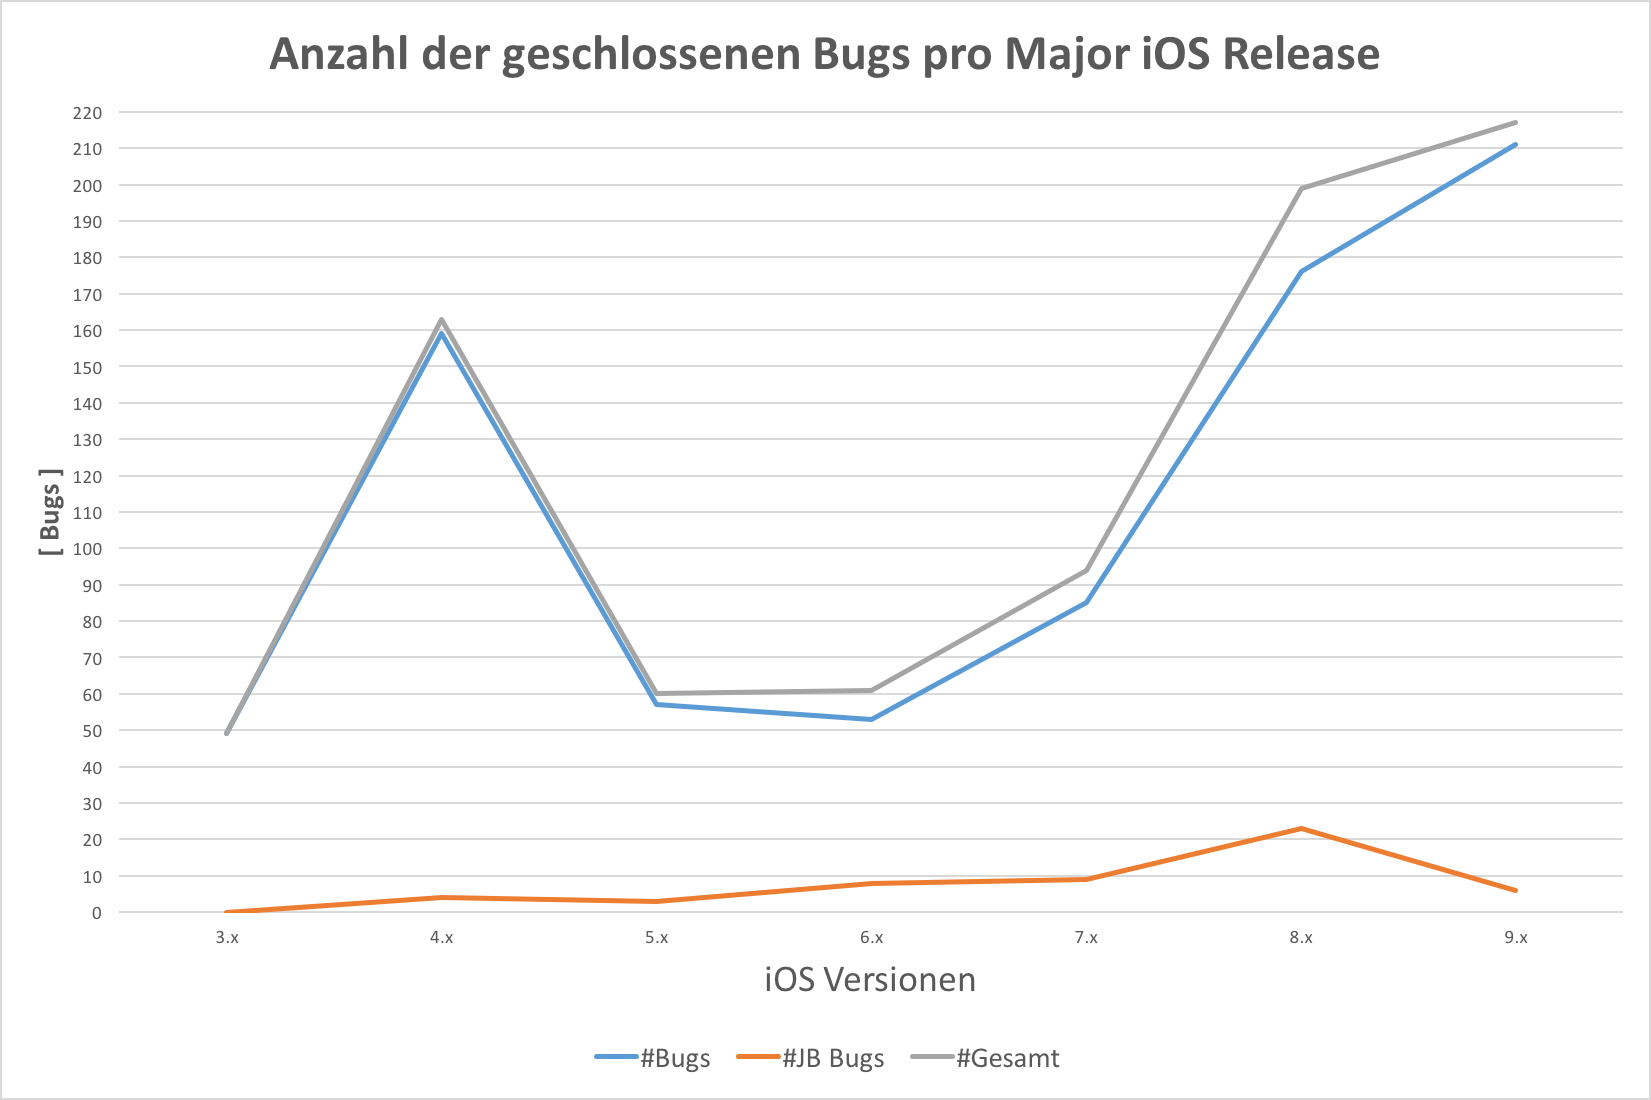
\includegraphics[scale=0.45]{Bilder/SecUpdateMajor.png}
        \caption{Anzahl Bugs pro iOS Major Release}
        \label{fig:SecUpdateMajor}
\end{figure}

\section{Analyse des Ziels G1.1}
\label{sec:AnalyseG11}
% G1.1: Erstes abgeleitetes Ziel ist es, einen Zusammenhang zwischen der Sicherheit und der Vertrauenswürdigkeit des iOS Device und der verwendeten Hardware der iOS Geräte herzustellen.
 Die Hardware der iOS Produkte spielt bei der Sicherheit des iOS Device nur eine begrenzte Rolle. Die Daten in den Kapiteln \ref{sec:Frage1iOSVersion} und \ref{sec:Frage1SecureEnclave} zeigen diesen Sachverhalt ganz klar.\par  
Die Secure Enclave verbesserte die Vertraulichkeit des iOS Device. Da die gesamten kryptographischen Verfahren für die File Keys, die Daten für den FingerPrint und vieles mehr in der Trust Zone des AMD Prozessors gespeichert werden. \par
Zu diesem Thema muss noch gesagt werden, dass die iOS Produkte ein in sich geschlossenes System sind, dies bedeutet der User kann weder die Hardware des Systems noch das Betriebssystem verändern. Alle Komponenten passen perfekt zueinander und sind aufeinander abgestimmt . Das iOS wurde für die Hardware des iOS Devices entwickelt und abgestimmt. Dies bringt Vorteil gegenüber anderen mobilen Betriebssystemen wie z.B. Android.  

\begin{description}
    \item[\parbox{\textwidth} {Zum heutigen Zeitpunkt sind drei iOS Devices als nicht sicher einzustufen}]~\par
    \begin{enumerate}
        \item iPhone - letzte unterstützte iOS Version 3.1.3
        \item iPhone 3G - letzte unterstützte iOS Version 4.2.1
        \item iPhone 3GS - letzte unterstützte iOS Version 6.1.6
    \end{enumerate}
\end{description} 
 
 
\section{Analyse des Ziels G1.2}
\label{sec:AnalyseG12}

%G1.2: Zweites abgeleitetes Ziel dieser Arbeit ist es, einen Zusammenhang zwischen der Sicherheit und der Vertrauenswürdigkeit des iOS Device und der installierten iOS Software herzustellen.

Die erhobenen Daten zeigen, dass die Sicherheit des Systems neben dem verwendeten Passcode, der iOS Konfiguration, dem iOS selbst noch von einem Faktor massiv abhängt den regelmäßigen Sicherheitsupdates.  
\begin{description}
    \item[\parbox{\textwidth} {Bei der Konfiguration sind folgende Konfigurationsparameter anzuführen}]~\par
    \begin{itemize}
       \item die Anzahl der Passcodestellen
       \item die Aktivierung des Parameters \textit{\glqq Daten löschen\grqq{}}. Das hat zur Folge, dass nach zehn falschen Eingaben des Passcode alle Daten des iOS Device gelöscht werden.
    \end{itemize}
\end{description} 

Apple veröffentlicht bis zum heutigen Datum (18.7.2016) für die iOS Major Release 9.x neun Sicherheitsupdates. Diese Sicherheitsupdates schlossen insgesamt 217 Bugs. Sechs dieser Bugs wurden für das JB Pangu verwendet.  Seit der iOS Version 3.x wurden insgesamt 843 Softwarefehler in 49 Sicherheitsupdates geschlossen. 55 dieser Softwarefehler wurden von JB-Tools verwendet. Eine genaue Auflistung der Daten ist in der Tabelle \ref{tab:AppleReaktionszeitAll} und in den Abbildungen \ref{fig:AnalyseiOSSicherheitsupdate3}, \ref{fig:AnalyseiOSSicherheitsupdate5}, \ref{fig:AnalyseiOSSicherheitsupdate5}, \ref{fig:AnalyseiOSSicherheitsupdate7}, \ref{fig:AnalyseiOSSicherheitsupdate8} und \ref{fig:AnalyseiOSSicherheitsupdate9} ersichtlich.

Die Daten lassen vermuten, dass Apple gezielt JB-Tools „Reverse Engineering“ und die die für das JB verwendeten Sicherheitslücken der iOS Version schließt.
\section{Analyse des Ziels G1}
\label{sec:AnalyseG1}

Das iOS Device gehört zu den sichersten mobilen Geräten auf dem freien Markt. Die iOS Update-Funktionalität ist im iOS Betriebssystem integriert. Der User wird in regelmäßigen Abständen daran erinnert, dass eine neue iOS Version zur Verfügung steht. Somit wird der User aktiv animiert die iOS Version auf sein Gerät aktuell zuhalten.  Bei Android muss sich der User selbst für die Softwareaktualisierung verantwortlich.\par
 
Im Vergleich zu Android veröffentlicht Apple weit mehr Sicherheitsupdates pro Jahr. Daraus kann einerseits geschlossen werden, dass die iOS Versionen aufgrund der Mehrzahl an Bugs als unsicherer einzustufen sind. Die andere Sichtweise ist, dass unter iOS mehr Codeanalysen durchgeführt werden. Ich schließe mich der zweiten Aussage an, da aufgrund der JBs mehr Aufmerksamkeit auf die Zeitnahen Sicherheitsupdates gelegt wird. Da es zu einem Imageverlust führt würde, wenn Sicherheitslücken zu lange ausgenutzt werden können. \par
Ein interessantes Detail ist noch anzuführen, die im Laufe der Jahre eingeführten Sicherheitsmechanismen wie zum Beispiel, ALSR, MAC und Sandbox hatten keine markanten Einfluss auf die Anzahl an Tagen die benötigt wurden um ein JB zu veröffentlichen. In den Abbildungen 5.2 und 5.3 gibt es keine Ausreißer in den Metriken. Erwarte hätte ich mir, dass zwischen der iOS Version 2.0 und 4.3 die Anzahl an Tagen bis ein JB veröffentlicht wurde massiv ansteigt.  Es gab nur eine markante Stelle. Die iOS Version 3.1.2 zeigt einen massiven Anstieg der Anzahl an Tagen die benötigt wurden um die untethered JBs JailbreakMe 2.0 und Spirit zu veröffentlicht . Dies ist aber darauf zurückzuführen, dass in den iOS Releases 3.1 und 3.1.1 Bugs geschlossen wurden,  die den untethered JB der vorhergehenden JBs ermöglichten. Ein tethered JB war für die iOS 3.1.2 nach XX Tagen verfügbar.\par
 
In Bezug auf JBs kann gesagt werden, dass ein installierter JB die Sicherheit und Vertrauenswürdig des Systems reduziert. Da Sicherheitsmechanismen von Apple eingeschränkt und/oder ausgeschalten werden. Der normale User ist sich über diese Konsequenzen nicht im Klaren und verfügt meisten nicht über das Wissen, das Device wieder sicher zu machen.

%----------------------------------------------------------------
%  File    :  chapter7.tex
%
%  Authors : Michael Fuska, FH Campus Wien, Austria
%
%  Created : 13 Feb 2016
%
%  Changed :  
% 
%----------------------------------------------------------------

\chapter{SSH Damon iOS}
\label{ch:ssh}

\section{Allgemein}
\label{sec:InstallSSH}


Hier wird analysiert wieviele JB iOS Devices den ssh Damon installiert haben
im 2ten schritt wird festgehalten wie oft das standard pw alpine verwendet wird

in dieses chapter werden auch die bestehenden SSH Malware eingegangen ...
iKee, Duh, 
iSAM

% https://www.theiphonewiki.com/wiki/Malware_for_iOS          %SSH Part
%----------------------------------------------------------------
%
%  File    :  chapter8.tex
%
%  Authors : Michael Fuska, FH Campus Wien, Austria% 
%  Created : 13 Feb 2016
%
%  Changed :  
% 
%----------------------------------------------------------------

\chapter{Conclusion}
\label{ch:Conclusion}
Apple versucht die  Anforderungen \textit{\glqq usability\grqq{}} und \textit{\glqq security\grqq{}} in ihren iOS Produkten zu vereinen. Das ist eine der Begründungen für die restriktiven Sicherheitsmechanismen von Apple. Die iOS Produkte sind ein geschlossenes System. Dies bedeutet, dass weder die Hardware noch die Software vom User verändert werden können. Dies ist auch ein Grund für die Stabilität der iOS Produkte. Ein weiterer Grund ist die simple Konfiguration des iOS Systems. Der User benötigt keine Vorkenntnisse, um eine sichere iOS Konfiguration vorzunehmen. Die Default-Konfiguration des iOS Device ist als sicher anzusehen. Nur die Passcode Konfiguration sollte von vier Digits auf sechs Digits verändert werden, da die gesamte Sicherheit des Systems von dem verwendeten Passcode abhängt, inklusive der Datenverschlüsselung des iOS Gerätes. \par 

\begin{description}
    \item[\parbox{\textwidth} {Die Sicherheit und Vertrauenswürdigkeit eines mobilen Gerätes hängt von mehreren Faktoren ab}]~\par
    \begin{enumerate}
        \item Dem Passcode, der zum Entsperren des Gerätes verwendet wird.
        \item Den Apps, die auf dem Gerät installiert wurden. 
        \item Der Verschlüsselung, die verwendet wird, um die Daten des Gerätes zu verschlüsseln.
        \item Den Sicherheitsmechanismen, die im mobilen Betriebssystems umgesetzt wurden.
        \item Den regelmäßigen Sicherheitsupdates, die dazu verwendet wurden, um die Sicherheitslücken des mobilen Betriebssystem zu schließen.  
    \end{enumerate}
\end{description} 
Installiert nun der User auf seinen iOS Device ein JB, so verlässt der User freiwillig die sichere iOS Umgebung. Die Installation eines JBs hat einen massiven Einfluss auf die Sicherheit und auf die Vertrauenswürdigkeit des iOS Systems. Ein JB erlaubt es, dass Apps mit einem selbst signierten Zertifikat auf dem iOS Device installiert werden können. Es liegt in der Hand des Users abzuschätzen, inwieweit er dem Hersteller der Apps vertraut, die er auf seinem iOS Device installieren möchte. Diese Apps wurde nicht auf Malware geprüft, und somit ist die Installation der Apps ein Glücksspiel. Die Sicherheitsanalysen zeigen, dass die meisten Viren auf einem iOS Device nur funktionieren, wenn ein JB auf dem Gerät installiert wurde. Ein Beispiel dafür ist die Malware KeyRaider \cite{KeyRaider}. Diese Malware funktioniert nur auf einem \textit{\glqq gejailbreaked\grqq{}} iOS Device und wird mit einer App installiert, die über Cydia heruntergeladen wurde. \par 
 Ein weiterer Punkt, der in diesem Zusammenhang angeführt werden muss, ist, dass die Konfiguration mancher Apps Fachwissen benötigt. Der User muss sich bewusst sein, welche Seiteneffekte diese Installation haben kann. Nach der Installation eines JBs haben alle iOS Devices dasselbe root-Passwort und der User muss dieses ändern. Der Virus \textit{\glqq ikee\grqq{}} basiert genau darauf, dass der User sein root-Passwort nicht geändert hat. Der Virus konnte sich am iOS Device einloggen, und persönliche Daten konnten verändert werden.\par 
 
Das ist die eine Seite des JBs, die andere Seite ist, dass durch \textit{\glqq Reverse Engineering\grqq{}} der JB-Tools die Sicherheitslücken in der iOS Software geschlossen werden. Die Sicherheitsupdates zeigen, dass einige Sicherheitslücken nur auf Grund der JBs geschlossen wurden. Da Apple durch den öffentlichen Druck \textit{\glqq gezwungen\grqq{}} wird, die Bugs der iOS Versionen zu schließen. Dieser Druck entsteht dadurch, dass für die Öffentlichkeit die Unsicherheit des iOS Devices \textit{\glqq sichtbar\grqq{}} gemacht wird. 



          %Conclusion

%-----

\appendix
% --- Verzeichnisse ------------------------------------------------------

\newpage
\chapter{Verzeichnisse}

% --- List of Figures ----------------------------------------------------

\newpage
\phantomsection
\addcontentsline{toc}{section}{Abbildungsverzeichnis}
\listoffigures



% --- List of Tables -----------------------------------------------------

\newpage
\phantomsection
\addcontentsline{toc}{section}{Tabellenverzeichnis}
\listoftables

% --- List of Listings -----------------------------------------------------

\newpage
\phantomsection
\addcontentsline{toc}{section}{Listings}
\lstlistoflistings

% --- Bibliography ------------------------------------------------------

\bibliographystyle{alpha}

% List references I definitely want in the bibliography,
% regardless of whether or not I cite them in the thesis.

\newpage
\phantomsection
\addcontentsline{toc}{section}{Literaturverzeichnis}
\bibliography{thesis}          % Appendix A

\end{document}

